\documentclass[10pt]{amsart}
\usepackage{amsmath}
\usepackage{amssymb}
\usepackage{amsthm}
%\usepackage{MnSymbol}
\usepackage{bm}
\usepackage{accents}
\usepackage{mathtools}
\usepackage{tikz}
\usetikzlibrary{calc}
\usetikzlibrary{decorations.pathmorphing,shapes}
\usetikzlibrary{automata,positioning}
\usepackage{tikz-cd}
\usepackage{forest}
\usepackage{braket} 
\usepackage{listings}
\usepackage{mdframed}
\usepackage{verbatim}
\usepackage{physics2}
\usephysicsmodule{ab,ab.legacy,diagmat,xmat,op.legacy}
\usepackage{derivative}
\usepackage{fixdif}
\usepackage{stmaryrd}
% \usepackage{euscript} 
\usepackage{eucal}
\usepackage{stackengine} 
%\usepackage{/home/patrickl/homework/macaulay2}

%font
% \usepackage[sc]{mathpazo}
% \usepackage{inconsolata}
\usepackage{microtype}
% \usepackage{fontspec} 
% \setmainfont{Tex Gyre Pagella}
% \usepackage[OT1,euler-digits]{eulervm}
% \usepackage{euler-math} 
% \usepackage[scaled=0.86]{berasans}
% \let\sffamilyold\sffamily
% \def\sffamily{\fontencoding{T1}\sffamilyold}
% \setmonofont{Inconsolatazi4}

%CS packages
\usepackage{algorithmicx}
\usepackage{algpseudocode}
\usepackage{algorithm}

% typeset and bib
\usepackage[english]{babel} 
% \usepackage[utf8]{inputenc} 
% \usepackage[T1]{fontenc}
% \usepackage[backend=biber,style=alphabetic,maxalphanames=4,maxnames=5,hyperref]{biblatex}
\usepackage[bookmarks, colorlinks, breaklinks]{hyperref} 
\hypersetup{linkcolor=blue,citecolor=magenta,filecolor=black,urlcolor=blue}
\usepackage{cleveref}
\crefname{equation}{}{}
\usepackage{graphicx}
\graphicspath{{./}}


% other formatting packages
\usepackage{float}
\usepackage{booktabs}
\usepackage[shortlabels]{enumitem}
\setitemize{noitemsep}
\usepackage{csquotes}
%\usepackage{titlesec}
%\usepackage{titling}
%\usepackage{fancyhdr}
%\usepackage{lastpage}
% \usepackage{parskip}
\newlist{mydescription}{description}{1}
\setlist[mydescription]{style=nextline,
                        font=\bfseries,
                        % Tweak the next 4 options as needed:
                        labelindent=1cm, 
                        leftmargin =2cm,
                        rightmargin=1cm,
                        topsep     =1ex
                       }

\usepackage{lipsum}

% delimiters
\DeclarePairedDelimiter{\gen}{\langle}{\rangle}
\DeclarePairedDelimiter{\floor}{\lfloor}{\rfloor}
\DeclarePairedDelimiter{\ceil}{\lceil}{\rceil}


\newtheorem{thm}{Theorem}[section]
\newtheorem{cor}[thm]{Corollary}
\newtheorem{prop}[thm]{Proposition}
\newtheorem{lem}[thm]{Lemma}
\newtheorem{conj}[thm]{Conjecture}
\newtheorem{quest}[thm]{Question}
\newtheorem{claim}[thm]{Claim}

\theoremstyle{definition}
\newtheorem{defn}[thm]{Definition}
\newtheorem{defns}[thm]{Definitions}
\newtheorem{con}[thm]{Construction}
\newtheorem{exm}[thm]{Example}
\newtheorem{exms}[thm]{Examples}
\newtheorem{notn}[thm]{Notation}
\newtheorem{notns}[thm]{Notations}
\newtheorem{addm}[thm]{Addendum}
\newtheorem{exer}[thm]{Exercise}

\theoremstyle{remark}
\newtheorem{rmk}[thm]{Remark}
\newtheorem{rmks}[thm]{Remarks}
\newtheorem{warn}[thm]{Warning}
\newtheorem{sch}[thm]{Scholium}


% unnumbered theorems
\theoremstyle{plain}
\newtheorem*{thm*}{Theorem}
\newtheorem*{prop*}{Proposition}
\newtheorem*{lem*}{Lemma}
\newtheorem*{cor*}{Corollary}
\newtheorem*{conj*}{Conjecture}

% unnumbered definitions
\theoremstyle{definition}
\newtheorem*{defn*}{Definition}
\newtheorem*{exer*}{Exercise}
\newtheorem*{defns*}{Definitions}
\newtheorem*{con*}{Construction}
\newtheorem*{exm*}{Example}
\newtheorem*{exms*}{Examples}
\newtheorem*{notn*}{Notation}
\newtheorem*{notns*}{Notations}
\newtheorem*{addm*}{Addendum}


\theoremstyle{remark}
\newtheorem*{rmk*}{Remark}

% shortcuts
\newcommand{\Ima}{\mathrm{Im}}
\newcommand{\A}{\mathbb{A}}
\newcommand{\G}{\mathbb{G}}
\newcommand{\N}{\mathbb{N}}
\newcommand{\R}{\mathbb{R}}
\newcommand{\C}{\mathbb{C}}
\newcommand{\Z}{\mathbb{Z}}
\newcommand{\Q}{\mathbb{Q}}
\newcommand{\E}{\mathbb{E}}
\renewcommand{\k}{\Bbbk}
\renewcommand{\L}{\mathbb{L}}
\renewcommand{\P}{\mathbb{P}}
\newcommand{\M}{\mathcal{M}}
\newcommand{\Mbar}{\overline{\mathcal{M}}}
\newcommand{\g}{\mathfrak{g}}
\newcommand{\h}{\mathfrak{h}}
\newcommand{\n}{\mathfrak{n}}
\renewcommand{\b}{\mathfrak{b}}
\newcommand{\ep}{\varepsilon}
\newcommand*{\dt}[1]{%
   \accentset{\mbox{\Huge\bfseries .}}{#1}}
%\renewcommand{\abstractname}{Official Description}
\newcommand{\mc}[1]{\mathcal{#1}}
\newcommand{\T}{\mathbb{T}}
\newcommand{\mf}[1]{\mathfrak{#1}}
\newcommand{\mbf}[1]{\mathbf{#1}}
\newcommand{\bv}{\mbf{v}}
\newcommand{\bq}{\mbf{q}}
\newcommand{\bp}{\mbf{p}}
\newcommand{\ut}{\ul{t}}
\newcommand{\uz}{\ul{z}}
\newcommand{\ur}{\ul{j}}
\newcommand{\btau}{\bm{\tau}}
\newcommand{\mr}[1]{\mathrm{#1}}
\newcommand{\on}[1]{\operatorname{#1}}
\newcommand{\ms}[1]{\mathsf{#1}}
\newcommand{\mt}[1]{\mathtt{#1}}
\newcommand{\ol}[1]{\overline{#1}}
\newcommand{\ul}[1]{\underline{#1}}
\newcommand{\wt}[1]{\widetilde{#1}}
\newcommand{\wh}[1]{\widehat{#1}}
\renewcommand{\div}{\operatorname{div}}
\newcommand{\1}{\mathbf{1}}
\newcommand{\2}{\mathbf{2}}
\newcommand{\3}{\mathbf{3}}
\newcommand{\I}{\mathrm{I}}
\newcommand{\II}{\mr{I}\hspace{-1.3pt}\mr{I}}
\newcommand{\III}{\mr{I}\hspace{-1.3pt}\mr{I}\hspace{-1.3pt}\mr{I}}
\renewcommand{\v}{\mbf{v}}
\newcommand{\w}{\mbf{w}}
\newcommand{\bmu}{\bm{\mu}}
\newcommand{\pre}{\mr{pre}}
\newcommand{\vir}{\mr{vir}}
\newcommand{\red}{\mr{red}}
\newcommand{\fl}{\mr{fl}}
\newcommand{\ps}[1]{\llbracket #1 \rrbracket}
\newcommand{\ls}[1]{\llparenthesis #1 \rrparenthesis}
\newcommand{\GW}{\ms{GW}}
\newcommand{\LG}{\ms{LG}}
\newcommand{\IIA}{\ms{IIA}}
\newcommand{\IIB}{\ms{IIB}}
\newcommand{\QM}{\ms{QM}}
\newcommand{\cs}{\ms{cs}}

\DeclareMathOperator{\Der}{Der}
\DeclareMathOperator{\Tor}{Tor}
\DeclareMathOperator{\Hom}{Hom}
\DeclareMathOperator{\End}{End}
\DeclareMathOperator{\Ext}{Ext}
\DeclareMathOperator{\ad}{ad}
\DeclareMathOperator{\Aut}{Aut}
\DeclareMathOperator{\Rad}{Rad}
\DeclareMathOperator{\Pic}{Pic}
\DeclareMathOperator{\NS}{NS}
\DeclareMathOperator{\supp}{supp}
\DeclareMathOperator{\Supp}{Supp}
\DeclareMathOperator{\depth}{depth}
\DeclareMathOperator{\sgn}{sgn}
\DeclareMathOperator{\spec}{Spec}
\DeclareMathOperator{\Spec}{Spec}
\DeclareMathOperator{\proj}{Proj}
\DeclareMathOperator{\Proj}{Proj}
\DeclareMathOperator{\ord}{ord}
\DeclareMathOperator{\Div}{Div}
\DeclareMathOperator{\Bl}{Bl}
\DeclareMathOperator{\coker}{coker}
\DeclareMathOperator{\ev}{ev}
\DeclareMathOperator{\st}{st}
\DeclareMathOperator{\pr}{pr}
\DeclareMathOperator{\ch}{ch}
\DeclareMathOperator{\Cont}{Cont}
\DeclareMathOperator{\Crit}{Crit}

% \addbibresource{../../notes/math.bib}

\title[Higher-genus GW of compact CY3]{Notes on the higher-genus Gromov-Witten theory of compact Calabi-Yau threefolds}
\author{Patrick Lei}
\date{January 2025}
\allowdisplaybreaks

\begin{document}
    
\begin{abstract}
    These notes, taken during the first two weeks of the program \href{https://scgp.stonybrook.edu/archives/42649}{Recent developments in higher genus curve counting} at the Simons Center for Geometry and Physics, explain how to prove important structural results in the higher-genus Gromov-Witten theory of compact Calabi-Yau threefolds. 
\end{abstract}

\maketitle

\tableofcontents

\section{Introduction}%
\label{sec:Introduction}

One of the oldest problems in Gromov-Witten theory is to compute the Gromov-Witten invariants of compact Calabi-Yau threefolds. While there are a variety of physical methods which have allowed physicists to make spectacular predictions in a wide range of examples, mathematical progress has often been frustratingly slow due to a lack of satisfactory tools to attack the problem with. To illustrate this, we will briefly outline some developments in mathematics regarding Calabi-Yau threefolds with $h^2 = 1$ which arise as complete intersections in weighted projective space.
\begin{itemize}
    \item For complete intersections in projective space, a genus-zero mirror theorem was proved by Givental in 1996 and Lian-Liu-Yau in 1997.
    \item For complete intersections in weighted projective space, a genus-zero mirror theorem was proved by Coates-Corti-Lee-Tseng in 2006 in the convex case and by Jun Wang in 2019 in the non-convex case. The main difficulty in the non-convex case is the failure of the quantum Lefschetz theorem, which is the main tool used in the work of Givental, LLY, and CCLT.
    \item Meanwhile, a genus-one mirror theorem was proved for the quintic by Zinger in 2007 and for complete intersections in projective space by Popa in 2010. This used the theory of reduced invariants developed by Vakil-Zinger, Li-Zinger, and various other authors, which is a technique of performing birational modifications to the main component of the moduli space of stable maps to force the quantum Lefschetz theorem to hold so that computations can be performed using virtual localization. Unfortunately, to this date no computations have been successfully performed using reduced invariants since.
    \item Another way to force the quantum Lefschetz theorem to hold is to consider the theory of GLSMs, which were constructed by various authors during the 2010s. Unfortunately, the virtual cycle is supported on the moduli space of stable maps to the threefold, which does not carry a torus action.
    \item For the quintic, the ambient space of the relevant GLSM is the total space of $\mc{O}_{\P^4}(-5)$. A cheap way to gain a torus action is to compactify the moduli space at infinity and consider relative (or logarithmic) invariants. This leads to the theory of logarithmic GLSMs, which was introduced by Chen-Janda-Ruan in 2019. Before this, Guo-Janda-Ruan used this theory, including a still conjectural virtual localization formula, to prove a genus-two mirror theorem for the quintic in 2017 (up to the fact that the moduli space used in their 2017 paper is still not defined) and to prove the Yamaguchi-Yau finite generation conjecture, holomorphic anomaly equations, and orbifold regularity (as well as the conifold gap condition in low genus) for the quintic.
    \item Because a GLSM is an enumerative theory of a critical locus in a GIT quotient, it depends on a stability parameter. We can vary the stability parameter and construct a master theory following the master space construction of Thaddeus. This leads to the theory of Mixed-Spin-P fields, which was first constructed by Chang-Li-Li-Liu in 2015 (for the quintic only). Unfortunately, the original theory is impossible to compute with when $g \geq 2$, so a parameter $N$ was introduced by Chang-Guo-Li-Li in 2018. In the same year, Chang-Guo-Li proved the Yamaguchi-Yau finite generation conjecture, BCOV Feynman rule, and holomorphic anomaly equations for the quintic threefold. These results were generalized to hypersurfaces in weighted projective space by the author in 2024.
    \item A genus-one mirror theorem for hypersurfaces in weighted projective space was finally proved in 2024 by the author using the theory of Mixed-Spin-P fields.
    \item The Castelnuovo bound was proved in 2022 by Liu-Ruan for any Calabi-Yau threefold satisfying a conjectural Bogomolov-Gieseker-type inequality (which includes the quintic threefold) due to Bayer-Macri-Toda and a weaker version of the result was proved by Zhiyu Liu in 2024 without assuming the conjectural inequality. These results were obtained using the GW/DT correspondence, which was proved for complete intersections in products of projective spaces by Pandharipande-Pixton in 2012 and for all Calabi-Yau threefolds by Pardon in 2023.
\end{itemize}

These notes are about the techniques, namely log GLSMs and MSP fields, used to prove the most important conjectures which are provided to us by physicists, namely the Yamaguchi-Yau finite generation conjecture and the holomorphic anomaly equations.~\Cref{pt:prelim} covers the B-model topological string and the Givental formalism,~\Cref{pt:logglsm} covers log GLSMs, and~\Cref{pt:msp} covers Mixed-Spin-P fields. We will cover both the foundational theory and the calculations in both approaches. 

\subsection*{Author's note}%
\label{sub:Disclaimer}

In contrast to the genus zero situation, not much is known about higher-genus Gromov-Witten theory. This is in part because there are significantly fewer tools to study higher-genus invariants, and the ones which do exist seem to be considered extremely inaccessible. It is my sincere hope that these notes can help make the subject more accessible. 

All errors are the sole responsibility of the author. Please email me if you find any mistakes or typos in these notes.

The names next to section titles indicate that the material in that part of the notes comes from talks given by that speaker. The notes from the lectures by Albrecht Klemm were taken partly during the lecture and partly by watching the videos on the SCGP website, the notes from my lectures are simply my lecture notes, and the notes from all other lectures were taken during the lecture, with some material being provided by the speakers after their lectures.

\subsection*{Acknowledgements}%
\label{sub:Acknowledgements}

I would like to thank Qile Chen, Felix Janda, Sheldon Katz, Melissa Liu, John Pardon, and Rachel Webb for organizing the program. I would also like to thank Konstantin Aleshkin, Shuai Guo, Melissa Liu, and Dimitri Zvonkine for helpful discussions regarding the material in my lectures. Further thanks goes to Qile Chen for generously providing the notes from his lectures, Felix Janda for pointing out some subtleties and correcting some errors related to the material in his lectures, Sheldon Katz for pointing out that the K\"ahler structure bundle is the dual of the Hodge bundle, and the Simons Center for posting videos of all of the lectures.


\part{Mathematical and physical preliminaries}
\label{pt:prelim}

\section{Introduction to the topological B-model (Albrecht Klemm)}%
\label{sec:Introduction to the topological B-model (Albrecht Klemm)}

\subsection{Mirror symmetry and the role of Calabi-Yau threefolds}%
\label{sub:Mirror symmetry and the role of Calabi-Yau threefolds}


Let $X(\Omega, \omega)$ be a Calabi-Yau $n$-fold, where here $\Omega$ is a holomorphic $n$-form and $\omega$ is a K\"ahler form. Recall that this is equivalent to having $SU(n)$ holonomy or to $K_X = 0$. By a result of Yau, there exists a K\"ahler-Einstein metric $g$ in the class of $\omega$ with vanishing Ricci curvature. For our purposes, we will mostly consider the case when $n=3$.

We will really consider Families of Calabi-Yau varieties
\[ \mc{X} \to X \to \mc{M}(\uz, \ut), \]
where $\mc{M}(\uz, \ut)$ is parametrized by a combination of complex structure moduli $\uz$ and K\"ahler structure moduli $\ut_{\R}$ complexefied by a Neveu-Schwarz harmonic $2$-form $B$ to $\ut$. We will denote the fiber by
\[ X(\Omega_{\uz}, \omega_{\ut}). \]

On the moduli of complex structures $\mc{M}(\uz)$, the tangent space $H^{(0,1)}(X,T_X)$ has a basis given by harmonic forms
\[ A^{(k)} = A_{\ol{i}}^{(k) j} \pdv{}{x^j} \d{x^{\ol{i}}} \]
for $k = 1, \ldots, h^{n-1,1}(X)$. Because we are in the Calabi-Yau setting, contracting with $\Omega$ gives us a basis
\[ \chi^{(k)} = A^{(k)} \lrcorner \Omega \]
of $H^{n-1,1}(X)$. By a theorem of Tian-Todorov, the moduli space is unobstructed. The B-model is built from mathematical structures on $\mc{M}(\uz)$.

There is a moduli space $\mc{M}_g$ parameterized by $\delta g$ subject to the condition
\[ R_{i\ol{j}} (g+\delta g) = 0. \]
To first order, we have
\[ \nabla^{\rho} \nabla_{\rho} \delta g_{\mu\nu} - 2 R_{\mu\nu}^{\kappa\sigma} \delta g_{k\sigma} = 0. \]
The indices with pure Hodge type correspond to harmonic forms in $H^{(0,1)}(X, TX)$ with components
\[ \delta g_{\ol{j}^{i}} = g^{i\ol{k}} \delta g_{\ol{k}\ol{j}} () \]
yielding the Kuranishi family over $\mc{M}(\uz)$.
The mixed indices correspond to real harmonic $(1,1)$-forms, and expanding the K\"ahler form linearly we obtain
\[ \omega = \sum t_{\R}^k \omega^{(k)} \]
in terms of real K\"ahler parameters
\[  \Re(t^k) = t_{\R}^k = \int_{\mc{C}_{(k)}} \omega > 0, \] which are volumes of holomorphic curves.

The K\"ahler moduli space $\mc{M}(\ut_{\R})$ is the real K\"ahler cone subject to positivity conditions from integration over $k$-dimensional holomorphic submanifolds, namely
\[ \int_{\mc{D}^{(k)}} \omega^{\wedge k} > 0. \]
The bosonic part of the string action contains the harmonic antisymmetric Neveu-Schwarz background field $b_{i\ol{j}}$
\[ S_{\ms{bos}} =\frac{1}{2\pi\alpha'} \int_{\Sigma} \sqrt{h} (h^{ab} g_{i\ol{j}} + \sqrt{-1} b_{i\ol{j}}\ep^{ab}) \partial_{\sigma_a} x^i \partial_{\sigma_b} x^{ \ol{j} }, \]
where $\alpha'$ is the string coupling constant. Its critical values measure complexified volumes of holomorphic curves by
\[ t^k = \int_{\mc{C}^k} (\omega + ib) = \Re(t^(k)) + \sqrt{-1} \Im(t^{(k)}). \]


\begin{conj}
    For non-rigid Calabi-Yau threefolds $X$ with $h^{2,1} > 0$, there exists a mirror Calabi-Yau $\hat{X}$ with $h^{1,1}(\hat{X})= h^{2,1}(x)$ and $h^{2,1}(\hat{X}) = h^{1,1}(X)$ such that the moduli spaces satisfy
    \[ \mc{M}[\hat{X}](\hat{\uz}) = \mc{M}[X](\ut) \qquad \text{and} \qquad \mc{M}[\hat{X}](\hat{\ut}) = \mc{M}[X](\uz) \]
    and all relevant physical and mathematical structures can be identified using locally invertible mirror maps
    \[ \hat{\uz}(\ut) \qquad \text{and} \qquad \hat{\ut}(\uz). \]
\end{conj}

Mirror symmetry identifies Type IIA compactifications on $X$ with Type IIB compactifications on $\hat{X}$, and vice versa. Additional Ramond-Ramond background fields and axio-dilaton fields with modulus $\ur$ and $a$ extend the moduli spaces as
\[ \mc{M}^{\IIB}[X] = \mc{M}[X](\uz) \times \mc{Q}[X](\ut, \ur, a) \]
and 
\[ \mc{M}^{\IIA}[\hat{X}] = \mc{M}[X](\hat{\ut}) \times \mc{Q}[\hat{X}](\hat{\uz}, \hat{\ur}, \hat{a}), \]
where $\mc{Q}$ denotes a quaternionic extension of $\mc{M}$. The RR $(k+1)$-form fields are sourced from $D_k$ branes. $k$ is even for Type IIA and odd for Type IIB. The $D_{2m}$ correspond to coherent sheaves and $D_{2m+1}$ correspond to special Lagrangian branes. Here, $\mc{Q}$ is the $4$d $N=2$ hyper-multiplet moduli space, and $\mc{M}$ is the $4$d $N=2$ vector multiplet moduli space.

One kind of mathematical structure is Hodge numbers. In the traditional picture of the Hodge diamond, Poincar\'e duality corresponds to a reflection along the horizontal axis, Dolbeaut symmetry is a reflection along the vertical axis, and mirror symmetry is a reflection along a line with slope $1$.

Superstring theory is defined by maps
\[ X \colon \Sigma_g \to \mc{C}_{\beta} \subset \text{spacetime} \]
weighted by an action $S$ which is a supersymmetric extension of the area of $\mc{C}_{\beta}$. It is easy to quaantize the Neveu-Schwarz-Ramond action, and the Green-Schwarz action incorporates the RR fields. The \textit{first quantized theory} is defined by a variatonal integral with partition function
\[ Z(g,b,\phi) = \int \mc{D}X \mc{D}h \mc{D}\psi_{\ms{ferm}} e^{\frac{i}{\hbar} S_{\ms{NSR}}(X,h,\psi_{\ms{ferm}},g,b,\phi)}. \]

Superstring theory is Weyl invariant in ten dimensions, or in other words
\[ \int \mc{D}h \to \sum_{g = 0} \int_{\mc{M}_{\Sigma_g}} \mu_{3g-3}, \]
so we obtain a discrete sum of finite-dimensional integrals. This implies that the compact part $X$ of the spacetime $M$ must be a complex threefold. If $X$ is Calabi-Yau, we obtain an extended $(2,2)$ world-sheet SCFT, which has four nilpotent operators
\[ Q_{\pm}^2 = \bar{Q}_{\pm}^2 = 0. \]
The $A$-twist corresponds to taking
\[ Q_A = Q_- + \bar{Q}_+ \]
and the $B$-twist corresponds to
\[ Q_B = \bar{Q}_- + \bar{Q}_+. \]
The topological $A$-model yields a cohomological topological theory depending only on the K\"ahler structure, while the topological $B$-model is a homological topological theory depending only on the complex structure. Mirror symmetry then exchanges the $A$-model and $B$-model.

\subsection{The topological A-model and B-model}%
\label{sub:The topological A-model}

In the $A$-model, terms depending on the complex structure are $Q_A$-exact, so the variatinoal integral simplifies to
\[ Z = \sum_{g=0}^{\infty} \sum_{\beta \in H_2(X,\Z)} g_s^{2g-2} Q^{\beta} \int_{\Mbar_g(X,\beta)} \1. \]
Here, we have
\[ Q = e^{2\pi i \int_{\mc{C}_{\beta}}i\omega+b} = e^{t\beta} \]
and these holomorphic maps are stationary points of the action. Moreover, taking the logarithm, we obtain
\[ \mc{F}(g_s, Q) = \log Z = \sum_{g,\beta} g_s^{2g-2} Q^{\beta} r_g^{\beta} = \sum_{g=0}^{\infty} g_s^{2g-2} \mc{F}_g(Q), \]
where $r_g^{\beta}$ are the GW invariants.
Rewriting these in terms of GV invariants, we obtain
\[ \mc{F}(g_s, Q) = \frac{c(t)}{\lambda^2} + \ell(t) + \sum_{g,\beta} \sum_{m=1}^{\infty} \frac{n_g^{\beta}}{m}\ab(2 \sin \frac{m g_s}{2})^{2g-2} Q^{m\beta}. \]


In the $B$-model, the terms depending on the K\"ahler structure are $Q_B$-exact and the variational integral localizes to constant maps albeit with a nontrivial measure depending on the complex structure. Mirror symmetry is supposed to be an exact duality, so we should have
\begin{align*}
    \ab<\mc{O}_i^{(0)} \mc{O}_j^{(0)} \mc{O}_k^{(0)}>_{g=0} &= \int_{\hat{X}} \Omega(z) \partial_{z_i} \partial_{z_j} \partial_{z_k} \Omega(z) \\
    &= \partial_{t_i} \partial_{t_j} \partial_{t_k} \mc{F}_0(t).
\end{align*}

Period integrals
\[ \Pi_{ij}(\uz) = \int_{\Gamma_i} \gamma^j(\uz) \]
define a nondegenerate pairing between middle homology and cohomology by Stokes' theorem. This pairing is antisymmetric if $n$ is odd and symmetric if $n$ is even. For example, if $X$ is a K3 surface, then the lattice $H^2(X,\Z)$ is
\[ E_8(-1)^{\oplus 2} \oplus \begin{pmatrix}
    0 & 1 \\
    1 & 0
\end{pmatrix}^{\oplus 3}.
\]
If $n$ is odd, we can fix an integral symplectic basis $\ul{\Gamma} = \{A_{\ell}, B^{\ell}\}$, which is defined only up to the action of $\mr{Sp}(b_n(X), \Z)$.

\begin{exm}
    If we consider an elliptic curve $p_3 = wy^2-x(x-w)(x-wz) = 0 \subset \P^2$, then we obtain
    \[ \Omega(z) = \oint \frac{2 \d{x} \wedge \d{y}}{p_3} = \frac{\d{x}}{y} \]
    and
    \[ \partial_z \Omega(z) \sim \frac{x\d{x}}{y}. \]
    Then the integrals 
    \[ E_1(z) = \oint_A \qquad \text{and} \qquad E_2(z) = \oint_B \Omega \]
    are elliptic integrals. The periods are annihilated by the Picard-Fuchs operator, and by definition thus satisfy the equation
    \[ \mc{L} \int_{\Gamma} \Omega = \ab[(1-z)\partial_z^2 + (1-2z) \partial_z - \frac{1}{4}] \int_{\Gamma} \Omega = 0. \]
\end{exm}

The main constraints which govern the periods of a Calabi-Yau $n$-fold are the Riemann bilinear relations
\[ e^{-K} = i^{n^2} \int_X \Omega \wedge \bar{\Omega} > 0. \]
This defines the exponential of the \textit{K\"ahler potential} $K(z)$ for the Weil-Petersson metric
\[ G_{i\bar{\jmath}} = \partial_{z_i} \bar{\partial}_{\bar{z}_{\bar{\jmath}}} K(z) \]
on $\mc{M}[X](\uz)$. There are also holomorphic bilinear relations
\[ \int_X \Omega \wedge \ul{\partial}_{\ell_k}^k \Omega = \begin{cases}
    0 & k < n \\
    C_{\ell_n}(z) & \ell = n
\end{cases}
\]
which follow from Griffiths transversality. Here, the integrand in the left hand side are arbitrary combinations of derivatives of $\Omega$ with respect to the $z_i$. We will see later that these give rise to propagators, the holomorphic anomaly equations, and other structures. The $C_{\ell_n}(z)$ are rational functions labelled by $\ell_n$ up to permutations.They are also determined by differential ideals $\mc{L}\vec{\Pi}$ also determine the $C_{\ell_n}(z)$ up to normalization.

\begin{rmk}
    In terms of the periods $\vec{\Pi}$, if we write them in a basis compatible with the intersection form $\Sigma$, the quantities in the relations may be written as
    \[ \int_X \Omega \wedge \bar{\Omega} = \vec{\Pi}^{\dag} \Sigma \vec{\Pi} \qquad \text{and} \qquad \int_X \Omega \wedge \ul{\partial}_{\ell_k}^k \Omega = - \vec{\Pi}^{\dag}\Sigma \ul{\partial}_{\ell_k}^k \vec{\Pi}. \]
\end{rmk}

\subsection{The quintic}%
\label{sub:The quintic}

Consider the mirror quintic $W$, which is given by the equation
\[ \hat{p}_5 = \sum_{i=0}^4 x_i^5 - 5 z^{-\frac{1}{5}} \prod_{k=0}^4 z_i = 0 \subset \hat{\P}^4. \]
The period vector $\Pi(z)$ (with an appropriate choice of integral cycles) fulfills the Picard-Fuchs equation
\[ \ab[\theta^4 - 5^5z \ab(\theta + \frac{1}{5})\ab(\theta + \frac{2}{5})\ab(\theta + \frac{3}{5})\ab(\theta + \frac{4}{5})] \Pi(z) = 0, \]
where $\theta = z \odv{}{z}$.

We want to find a basis where the monodromies around the singular points are integral symplectic matrices, so we look at the Riemann symbol and see that it is given by
\[ \mc{P}\ab\{ \begin{matrix}
    0 & 5^{-5} & \infty & * \\
    0 & 0 & \frac{1}{5} \\
    0 & 1 & \frac{2}{5} & z \\
    0 & 2 & \frac{3}{5} \\
    0 & 1 & \frac{4}{5}
\end{matrix}
\}.\]
Here, $z=0$ is a point of maximal unipotent monodromy, $z=\infty$ is the orbifold (or Landau/Ginzburg, or Gepner) point, and $z=5^{-5}$ is the conifold point. At a point of maximal unipotent monodromy, we can expand the mirror map and go to the large volume limit point in the $A$-model.

Using special geometry, Bryant and Griffiths showed that the periods may actually be expressed using a prepotential $\mc{F}$ as
\[ \begin{pmatrix}
    \int_{B_0} \Omega \\
    \int_{B_1} \Omega \\
    \int_{A_0} \Omega \\
    \int_{A_1} \Omega
\end{pmatrix} = \begin{pmatrix}
    F_0 \\
    F_1 \\
    X^0 \\
    X^1 
\end{pmatrix} = \begin{pmatrix}
    2 \mc{F}_0 - t \partial_t \mc{F}_0 \\
    \partial_t \mc{F}_0 \\
    1 \\ 
    t
\end{pmatrix}.
\]
These correspond to triple logarithmic, double logarithmic, analytic, and logarithmic solutions, respectively. Using this, we can make the identification
\[ \mc{F}(z) = \mc{F}_0(t(z)), \]
where the mirror map is given by
\[ t = \frac{X^1}{X^0} = \log(z) + \mc{O}(z). \]
This was generalized to multi-parameter models by Hosono et. al, who related the classical terms to CTC Wall data $\kappa = D^3$ and $\sigma = \frac{\kappa \mod{2}}{2}$ in the formula
\[ \mc{F} = - \frac{\kappa}{6} + \frac{\sigma}{2}t^2 + \frac{c_2 \cdot D}{24}t + \frac{\chi(M)}{2} \frac{\zeta(3)}{(2\pi i)^3} - \frac{1}{(2\pi i)^3}\sum_{\beta \neq 0} n_0^{\beta} \on{Li}_3(Q^{\beta}). \]
Later, we will use this to find the integral symplectic basis without calculating any monodromy.

We now turn our attention to calculating the numbers $n_g^{\beta}$. We already saw the genus-zero invariants, but we are also interested in the higher-genus ones. Some invariants in low genus and degree are given in~\Cref{tab:g0gvquintic}.
\begin{table}[htpb]
    \centering
    \caption{Low genus GV invariants of the quintic.}
    \label{tab:g0gvquintic}
    \begin{tabular}{cccccc}
        \toprule
        $g$ & $d=1$ & $d=2$ & $d=3$ & $d=4$ & $d=5$ \\
        \midrule
        $0$ & $2875$ & $609250$ & $317206375$ & $242467530000$ & $22930588887625$ \\
        $1$ & $0$ & $0$ & $609250$ & $3721431625$ & $12129909700200$ \\
        $2$ & $0$ & $0$ & $0$ & $534750$ & $75478987900$ \\
        $3$ & $0$ & $0$ & $0$ & $8625$ & $-15663750$ \\
        $4$ & $0$ & $0$ & $0$ & $0$ & $49250$ \\
        $5$ & $0$ & $0$ & $0$ & $0$ & $1100$ \\
        $6$ & $0$ & $0$ & $0$ & $0$ & $10$ \\
        \bottomrule
    \end{tabular}
\end{table}

Physical predictions were made by Candelas et. al for $g=0$, Bershadsky et al. for $g \leq 3$, and Huang et al. for $g \leq 53$.
The numbers $n_1^1$, $n_1^2$, and $n_1^3$ were calculated mathematically by Schubert, Katz, and Ellingsrud-Stromme, respectively. Kontsevich gave a mathematical proof of some numbers in $g=0$ before the genus-zero invariants were completely determined by Givental and Lian-Liu-Yau. The formula for the genus-one invariants was proved by Zinger.

\subsection{Fourteen one-parameter hypergeometric families}%
\label{sub:Fourteen one-parameter hypergeometric families}

There are fourteen hypergeometric Picard-Fuchs operators for one-parameter families of Calabi-Yau threefolds $\hat{X}$ given by
\[ \mc{L} = \theta^4 - \mu^{-1}z \prod_{k=1}^4 (\theta + a_k), \]
where the values of $\mu$ and $a_k$ are given in~\Cref{tab:oneparameter}.
\begin{table}[htpb]
    \centering
    \caption{Data of one-parameter hypergeometric families}
    \label{tab:oneparameter}
    \begin{tabular}{ccccccc}
        \toprule
        $N$ & $a_k$ & $\mu^{-1}$ & Mirror $X$ & $\kappa$ & $c_2 \cdot D$ & $\chi(X)$ \\
        \midrule
        $8$ & $\frac{1}{2},\frac{1}{2},\frac{1}{2},\frac{1}{2}$ & $2^8$ & $X_{2,2,2,2}(1^8)$ & $16$ & $64$ & $-128$ \\
        \\[-0.8em]
        $9$ & $\frac{1}{4},\frac{1}{3},\frac{2}{3},\frac{3}{4}$ & $2^63^3$ & $X_{4,3}(1^52^1)$ & $6$ & $48$ & $-156$ \\
        \\[-0.8em]
        $16$ & $\frac{1}{4},\frac{1}{2},\frac{1}{2},\frac{3}{4}$ & $2^{10}$ & $X_{4,2}(1^6)$ & $8$ & $56$ & $-176$ \\
        \\[-0.8em]
        $25$ & $\frac{1}{5},\frac{2}{5},\frac{3}{5},\frac{4}{5}$ & $5^5$ & $X_{5}(1^4)$ & $5$ & $50$ & $-200$ \\
        \\[-0.8em]
        $27$ & $\frac{1}{3},\frac{1}{3},\frac{2}{3},\frac{2}{3}$ & $3^6$ & $X_{3,3}(1^6)$ & $9$ & $54$ & $-144$ \\
        \\[-0.8em]
        $32$ & $\frac{1}{4},\frac{1}{4},\frac{3}{4},\frac{3}{4}$ & $2^{12}$ & $X_{4,4}(1^4 2^2)$ & $4$ & $40$ & $-144$ \\
        \\[-0.8em]
        $36$ & $\frac{1}{3},\frac{1}{2},\frac{1}{2},\frac{2}{3}$ & $2^4 3^3$ & $X_{3,2,2}(1^7)$ & $12$ & $60$ & $-144$ \\
        \\[-0.8em]
        $72$ & $\frac{1}{6},\frac{1}{2},\frac{1}{2},\frac{5}{6}$ & $2^{8}3^3$ & $X_{6,2}(1^53^1)$ & $4$ & $54$ & $-256$ \\
        \\[-0.8em]
        $108$ & $\frac{1}{6},\frac{1}{3},\frac{2}{3},\frac{5}{6}$ & $2^{4}3^6$ & $X_6(1^4 2^1)$ & $3$ & $42$ & $-204$ \\
        \\[-0.8em]
        $128$ & $\frac{1}{8},\frac{3}{8},\frac{5}{8},\frac{7}{8}$ & $2^{16}$ & $X_{8}(1^4 4^1)$ & $2$ & $44$ & $-296$ \\
        \\[-0.8em]
        $144$ & $\frac{1}{6},\frac{1}{4},\frac{3}{4},\frac{5}{6}$ & $2^{10}3^3$ & $X_{6,4}(1^3 2^2 3^1)$ & $2$ & $32$ & $-158$ \\
        \\[-0.8em]
        $200$ & $\frac{1}{10},\frac{3}{10},\frac{7}{10},\frac{9}{10}$ & $2^{8}5^5$ & $X_{10}(1^3 2^1 5^1)$ & $1$ & $34$ & $-288$ \\
        \\[-0.8em]
        $216$ & $\frac{1}{6},\frac{1}{6},\frac{5}{6},\frac{5}{6}$ & $2^{8}3^6$ & $X_{6,6}(1^2 2^2 3^2)$ & $1$ & $22$ & $-120$ \\
        \\[-0.8em]
        $864$ & $\frac{1}{12},\frac{5}{12},\frac{7}{12},\frac{11}{12}$ & $2^{12}3^6$ & $X_{12,2}(1^4 4^1 6^1)$ & $1$ & $46$ & $-484$ \\
        \bottomrule
    \end{tabular}
\end{table}
Here, the notation for the mirror $X$ means the complete intersection in the weighted projective space with weights given in parentheses with degrees given by the subscripts. The local exponents are all $0$ at the MUM point, $0,1,1,2$ at the conifold point $\mu$, and are given by $a_1, a_2, a_3, a_4$ at the orbifold point $\infty$. The monodromy around a singular point $*$ is captured by the minimal exponent\footnote{This corresponds to the degree of the base change needed to make the monodromy unipotent.} $1 \leq k < \infty$ such that
\[ (M_*^k-1)^{p+1} = 0 \]
for some $0 \leq p \leq \dim_{\C} X$. When $k > 1$ and $p=0$, then we have an orbifold point. When $p > 0$ we have an infinite shift monodromy. If $p=1$ and the local exponents take the form $a,b,b,c$, then we have a single vanishing period dual to a logarithmic degenerating period and hence a conifold point, and if the local exponents are take the form $a,a,b,b$, then we have two vanishing periods and two logarithmic degenerating periods, and this case is called a $K$-point. The case $p=2$ cannot occur by Schmid's $\on{SL}(2,\C)$ orbit theorem, and when $p=3$, we have a point of maximal unipotent monodromy with local exponents $a,a,a,a$.

At the point $z=0$, there is a Frobenius basis of solutions
\[ \Pi_0(z) = \begin{pmatrix}
    f_0(z) \\
    f_0(z) \log z + f_1(z) \\
    \frac{1}{2}f_0(z) (\log z)^2 + f_1(z) \log z + f_2(z) \\
    \frac{1}{6} f_0(z) (\log z)^3 + \frac{1}{2} f_1(z) (\log z)^2 + f_2(z)\log z + f_3 (z),
\end{pmatrix}
\]
where we normalize the power series to have $f_0(0) = 1$ and $f_{k>0}(0) = 0$. Therefore, we can find an integral basis
\[ \Pi = (2\pi i)^3 \begin{pmatrix}
    \frac{\zeta_3 \chi(M)}{(2\pi i)^3} & \frac{c_2 \cdot D}{24 \cdot 2\pi i} & 0 & \frac{\kappa}{(2\pi i)^3} \\
    \frac{c_2 \cdot D}{24} & \frac{\sigma}{2\pi i} & \frac{\kappa}{(2\pi i)^2} & 0 \\
    1 & 0 & 0 & 0 \\
    0 & \frac{1}{2\pi i} & 0 & 0
\end{pmatrix} \Pi_0.
\]
In the integral basis, all monodromies are integral symplectic matrices. At the point $z=0$, we have
\[ M_0 = \begin{pmatrix}
    1 & -1 & \frac{\kappa}{6} + \frac{c_2 \cdot D}{12} & \frac{\kappa}{6} + \sigma \\
    0 & 1 & \sigma - \frac{\kappa}{2} & -\kappa \\
    0 & 0 & 1 & 0 \\
    0 & 0 & 1 & 0
\end{pmatrix},
\]
and at the conifold point, we have
\[ M_{\mu} = \begin{pmatrix}
    1 & 0 & 0 & 0 \\
    0 & 1 & 0 & 0 \\
    -1 & 0 & 1 & 0 \\
    0 & 0 & 0 & -1
\end{pmatrix}.
\]
At $z=\infty$, we have $M_{\infty} = (M_0 M_{\mu})^{-1}$.

The work of Alexandrov-Feyzbakhsh-Klemm-Pioline-Schimannek solves the topological string on these models up to $g_{\ms{mod}}$ given in~\Cref{tab:stateofart} using $D_4$ brane and wall-crossing.\footnote{There have since been more improvements found by adding more $D_4$ brane charges.} Note that $g_{\ms{avail}}$ is the maximum genus for which data appears at~\url{http://www.th.physik.uni-bonn.de/groups/klemm/data.php} and $g_{\ms{integ}}$ is the maximum genus solved by the work of Huang-Klemm-Quackenbush. 
\begin{table}[htpb]
    \centering
    \caption{Current state of the art in physics literature as of January 2023.}
    \label{tab:stateofart}
    \begin{tabular}{cccccccc}
        \toprule
        $X$                   & $\chi_D$ & $n_1^p$ & $n_1^c$ & Type & $g_{\ms{integ}}$ & $g_{\ms{mod}}$ & $g_{\ms{avail}}$ \\
        \midrule
        $X_5(1^5)$            & $5$ & $7$ & $0$ & $O$ & $53$ & $69$ & $64$ \\
        $X_6(1^4 2^1)$        & $4$ & $4$ & $0$ & $O$ & $48$ & $66$ & $48$ \\
        $X_8(1^4 4^1)$        & $4$ & $4$ & $0$ & $O$ & $60$ & $84$ & $64$ \\
        $X_{10}(1^3 2^1 5^1)$ & $2$ & $7$ & $0$ & $O$ & $50$ & $70$ & $68$ \\
        $X_{4,3}(1^52^1)$     & $5$ & $9$ & $0$ & $O$ & $20$ & $24$ & $24$ \\
        $X_{6,4}(1^32^23^1)$  & $3$ & $3$ & $0$ & $O$ & $14$ & $17$ & $17$ \\
        $X_{3,3}(1^6)$        & $6$ & $14$ & $1$ & $K$ & $29$ & $33$ & $33$ \\
        $X_{4,4}(1^4 2^1)$    & $4$ & $6$ & $1$ & $K$ & $26$ & $34$ & $34$ \\
        $X_{6,6}(1^22^23^2)$  & $2$ & $1$ & $0$ & $K$ & $18$ & $21$ & $21$ \\
        $X_{6,2}(1^53^1)$     & $5$ & $7$ & $0$ & $C$ & $63$ & $84$ & $49$ \\
        $X_{4,2}(1^6)$        & $6$ & $15$ & $1$ & $C$ & $50$ & $64$ & $40$ \\
        $X_{3,2,2}(1^7)$      & $7$ & $21$ & $1$ & $C$ & $14$ & $?$ & $14$ \\
        $X_{2,2,2,2}(1^8)$    & $8$ & $33$ & $3$ & $M$ & $17$ & $?$ & $32$ \\
        \bottomrule
    \end{tabular}
\end{table}

\begin{rmk}
    Even inserting at least one $D_4$ brane requires going beyond the topological string, which only gives the usual DT or PT invariants (one $D_6$ brane, no $D_4$ branes, and arbitrary $D_2$ and $D_0$ brane charges). Hopefully, we will be able to explore the entire space of Bridgeland stability conditions in the future.
\end{rmk}

\subsection{More on periods}%
\label{sub:More on periods}

Consider the Picard-Fuchs operator
\[ \mc{L}^{(n+1)}(z) = \sum_{i=1}^{n+1} a_i(z) \partial_z^i \]
of a one-parameter Calabi-Yau $n$-fold with middle Hodge structure of type $1,1,\ldots, 1$. Defining the adjoint operator
\[ \mc{L}^{(n+1)\vee}(z) = \sum_{i=1}^{n+1}(-\partial_z)^i a_i(z), \]
then Griffiths transversality implies that the operator is essentially self-adjoint, or in other words
\[ \mc{L}^{(n+1)} C_{\uz} = (-1)^{n+1} C_{\uz} \mc{L}^{(n+1)\vee}. \]
Here, the Yukawa coupling $C_{\uz}$ satisfies the differential equation
\[ C_{\uz}' = -\frac{2}{n+1} a_n C_{\uz}. \]
For the quintic, we in fact obtain
\[ C_{zzz}= \frac{5}{z^3(1-5^5z)}. \]
Equivalently, self-adjointness implies
\[ \sum_{j=k}^{n+1} \binom{j}{k} \ab\{ \frac{C_{\uz}^{(j-k)}}{C_{\uz}} a_j + (-1)^{n+j}a_j^{j-k}\} = 0. \]
When $n=3$, this yields
\[ a_3^3 + 4a_3'' + 6a_3 a_3' + 8 a_1 - 4 a_2a_3 - 8 a_2' = 0. \]

In the multi-parameter case, the periods $\vec{\Pi}$ span the kernel of the Picard-Fuchs differential ideal
\[ \{ \mc{L}\} = \{ \mc{L}_k^{(d_k)} \mid k = 1,\ldots,\ell\} \]
generated by the differential operators
\[ \mc{L}_l^{(d_k)}(\ul{\theta}, \uz) \ul{\Pi}(\uz) = 0. \]
This system is complete if all three-point functions
\[ C_{ijk}(\uz) = C_{z_iz_jz_k}(\uz) \]
can be integrated from the Griffiths transversality relations.

\begin{exm}
    For the example $X_{18}(1^3 6^1 9^1)$ with middle Hodge structure $1,2,2,1$, the Picard-Fuchs equation is generated by
    \begin{align*}
        \mc{L}_1^{(2)} &= \theta_1 (\theta_1 - 3 \theta_2) - 12 z_1 (6 \theta_1 + 1) (6 \theta_1 + 5), \\
        \mc{L}_2^{(3)} &= \theta_2^3 + \prod_{i=0}^2 (3 \theta_2 - \theta_1 + i),
    \end{align*}
    and the $C_{ijk}$ are given by
    \begin{align*}
        C_{111} &= \frac{9}{z_1^3\Delta_1}; \\
        C_{112} &= \frac{3 \delta}{z_1^2 z_2 \Delta_1}; \\
        C_{122} &= \frac{\Delta_2^2}{z_1 z_2^2 \Delta_1}; \\
        C_{222} &= \frac{9(\delta^3 + (432z_1)^3)}{z_2^2 \Delta_1 \Delta_2},
    \end{align*}
    where the components of the discriminant are given by
    \[ \Delta_1 = (1-432z_1)^3 - 27z_2 (432z_1)^3 \qquad \text{and} \qquad \Delta_2 + 1 + 27 z_2, \]
    and $\delta = 1 - 432z_1$.
\end{exm}

If we shift the holomorphic form by
\[\Omega \to e^{f(z)} \Omega, \]
this induces a K\"ahler gauge transformation
\[ K \to K - f(z) - \ol{f(z)}. \]
Also note that the Yukawa couplings $C_{ijk}(\uz)$ are sections of
\[ \mc{L}^2 \otimes \on{Sym}^3 T^* \mc{M}(\uz)^{1,0}, \]
where $\mc{L}$ is the dual of the Hodge bundle.

By the local Torelli theorem, the $X^I$ components of the period vector
\[ \begin{pmatrix}
    \int_{B_0} \Omega \\
    \vdots \\
    \int_{B_r} \Omega \\
    \int_{A_0} \Omega \\
    \vdots \\
    \int_{A_r} \Omega
\end{pmatrix} = \begin{pmatrix}
    F_0 \\
    \vdots \\
    F_r \\
    X^0 \\
    \vdots \\
    X^r
\end{pmatrix}
\]
are homogeneous coordinates on $\mc{M}(\uz)$. Griffiths transversality implies that 
\[ F = \frac{1}{2}X^I F_I \in \mc{L}^2 \]
is a homogeneous prepotential such that 
\[ e^{-K} = i (F_i \bar{X}^I - X^I \bar{F}_I) \]
and the Yukawa couplings are given by
\[ C_{IJK} = \pdv{}{X^I}\pdv{}{X^J} \pdv{}{X^K} F. \]
Dividing by $X^0$, we will get inhomogeneous coordinates $t^i = \frac{X^i}{X^0}$, and we obtain the inhomogeneous prepotential
\[ \mc{F}(\ut) = \frac{F(X)}{(X^0)^2}. \]
The K\"ahler potential and Yukawa coupling become
\begin{align*}
    e^{-K} &= i [(t^{\bar{\imath}} - t^i)(\mc{F}_i + \mc{F}_{\bar{\imath}}) + 2 (\mc{F} - \bar{\mc{F}})] \\
    C_{ijk}(\ut) &= \partial_i \partial_j \partial_k \mc{F}(\ut).
\end{align*}
In addition, we have
\[ C_{ijk}(\ut) = \frac{1}{(X^0)^2} \pdv{z_{\ell}}{t^i} \pdv{z_m}{t^j}\pdv{z_n}{t^k} C_{\ell m n} (\uz). \]

In inhomogeneous coordinates, we can obtain the period vector from $\mc{F}(\ut)$ by
\[ \vec{\Pi}^T = X^0 (2 \mc{F}(\ut) - t^i \partial_i \mc{F}(\ut), \partial_i \mc{F}(\ut), 1, t^i). \]
The Picard-Fuchs equation is equivalent to the Gauss-Manin connection
\[ (\partial_i - A_i(\uz)) \vec{\Pi}(\uz) = 0, \]
where $i = 1,\ldots,r$ and $A_i(\uz) \in \Q[\uz]$. If we set
\begin{align*}
    \hat{\Omega}_0 &= \alpha_0 + t^i \alpha_i - \partial_i \mc{F}\beta^i -(2 \mc{F} -t^i \partial_i \mc{F}) \beta^0 \\
    \hat{\chi}_i &= \alpha_i - \partial_i \partial_j \mc{F} \beta^j - (\partial_a \mc{F} - t^i \partial_i \partial_j \mc{F})\beta^0 \\
    \hat{\chi}^i &= -\beta^i + t^a \beta^0 \\
    \hat{\Omega}^0 &= \beta^0,
\end{align*}
this becomes
\[ \partial_i \begin{pmatrix}
    \Omega_0 \\ \chi_j \\ \chi^j \\ \Omega^0
\end{pmatrix} = \begin{pmatrix}
    0 & \delta_i^k & 0 & 0 \\
    0 & 0 & C_{ijk}(\ut) & 0 \\
    0 & 0 & 0 & \delta_i^j \\
    0 & 0 & 0 & 0
\end{pmatrix} \begin{pmatrix}
    \Omega_0 \\ \chi_j \\ \chi^j \\ \Omega^0
\end{pmatrix}.
\]

\subsection{Special geometry}%
\label{sub:Special geometry}

On the moduli space of complex structures $\mc{M}_{\cs} \coloneqq \mc{M}(\uz)$, we have metric connections from the Weil-Petersson metric and the K\"ahler line bundle connection. On sections
\[ V_{j\bar{\jmath}} \in T^*_{1,0}\M_{\cs} \otimes T^*_{0,1}\M_{\cs} \otimes \mc{L}^{\otimes n} \otimes \bar{\mc{L}}^{\otimes m}, \]
the covariant derivatives are given by
\begin{align*}
    D_i V_{j\bar{\jmath}} &= \partial_i V_{j\bar{\jmath}} - \Gamma^{\ell}_{ij} V_{\ell\bar{\jmath}} + n K_i V_{j\bar{\jmath}} \\
    D^i V_{j\bar{\jmath}} &= \partial_{\bar{\imath}} V_{j\bar{\jmath}} - \Gamma^{\bar{\ell}}_{\bar{\imath}\bar{\jmath}} V_{i\bar{\ell}} + m K_{\bar{\imath}} V_{j\bar{\jmath}}.
\end{align*}
Using the covariant derivatives, we see that 
$\chi_i \in H^{n-1,1}(X)$ and $\bar{\chi}_{\bar{\imath}} \in H^{1,n-1}(X)$. 

Proceeding more systematically, repeated applications of $D_i$ yield
\begin{align*}
    D_i \Omega &= (\partial_i + K_i)\Omega = \chi_i \\
    D_i \chi_j &= -ie^{K} C_{ijk} G^{k\bar{k}}\chi_{\bar{k}} \\
    D_i \chi_{\bar{k}} &= G_{i\bar{k}} \bar{\Omega} \\
    D_i \bar{\Omega} &= 0.
\end{align*}
Using the relation
\[ [D_i, D_j] \chi_k = -G_{i\bar{\jmath}} \chi_k + R_{i\bar{\jmath}k}^p \chi_p, \]
we further deduce
\[ [D_i, D_{\bar{\jmath}}] \chi_k  = G_{k\bar{\jmath}} \chi_i - e^{2K} C_{\bar{\jmath}\bar{m}\bar{n}} G^{m\bar{m}} G^{n\bar{n}} C_{ikm} \chi_n. \]
It follows that
\[ [D_i, D_{\bar{\jmath}}]_{\ell}^k = -R_{i\bar{\jmath}\ell}^k = \partial_{\bar{\jmath}} \Gamma_{i\ell}^k = \delta_{\ell}^k G_{\bar{\jmath}i} + \delta_i^k G_{\bar{\jmath}\ell} - C_{\bar{\jmath}}^{km} C_{i\ell m}, \]
where $C_{\bar{\jmath}}^{k\ell} = e^{2K} C_{\bar{\jmath}\bar{k}\bar{\ell}} G^{k\bar{k}} G^{\ell\bar{\ell}}$. This equation is known as the \textit{special geometry equation} and is the integrability condition for the existence of the prepotential $\mc{F}$.

\subsection{Genus one predictions}%
\label{sub:Genus one predictions}

In a $(2,2)$ theory, the topological torus partition function is defined by
\[ F(t, \bar{t}) = \frac{1}{2} \int_{\mc{F}_{\ms{fund}}} \frac{\d^2 \tau}{\Im \tau} \Tr(-1)^F F_L F_R q^H \bar{q}^{\bar{H}} \]
as an integral of the fermion number projected partition function over the fundamental region of the torus. Using its relationship to the family index of Ray-Singer analytic torsion, it satisfies the holomorphic anomaly equation
\[ \partial_i \bar{\partial}_{\bar{\jmath}} F_1 = \frac{1}{2} C_{ijk} C_{\bar{\jmath}}^{k\ell} - \ab(\frac{\chi}{24}-1) G_{i\bar{\jmath}}. \]
Using $G_{i\bar{\jmath}} = \partial_{\bar{\jmath}} \partial_i K = \partial_{\bar{\jmath}} K_i$ and the special geometry equation, we can integrate the holomorphic anomaly equation to obtain
\begin{equation}\label{eqn:f1}
 F_1 = -\frac{1}{2} \log \det G_{i\bar{\jmath}} + \ab(\frac{1}{2}(h_{11}+1) - \frac{\chi}{24} + 1)K + \log f_1(z) + \log f_1(\bar{z}). 
\end{equation}

\subsection{Propagators}%
\label{sub:Propagators}

The \textit{propagators} are \textbf{an-holomorphic} sections $S^{ij}$, $S^i$, and $S$ of $\mc{L}^{-2}\otimes \on{Sym}^2(T\mc{M}_{\cs}^{1,0})$, $\mc{L}^{-2} \otimes T \mc{M}_{\cs}^{1,0}$, and $\mc{L}^{-2}$, respectively, defined by
\[ \partial_{\bar{\imath}} S^{jk} = C_{\bar{\imath}}^{jk}, \qquad \partial_{\bar{\jmath}} S^k = G_{i\bar{\jmath}} S^{ik}, \qquad \text{and} \qquad \partial_{\bar{\jmath}} S = G_{i\bar{\jmath}} S^i. \]
We can integrate the first equation using the special geometry equation and the observation that the only contributions to $C_{\bar{\jmath}}^{km} C_{i\ell m}$ are derivatives in $\bar{\partial}_{\bar{\jmath}}$. Therefore, if there exists an index $i$ such that $[C_{(i)}]_m$ is invertible, we obtain
\[ S^{km} = C^{(i)k\ell} (\delta_{\ell}^m K_{(i)} + \delta_{(i)}^m K_{\ell} + \Gamma^m_{(i)\ell} + q_{(i)\ell}^m), \]
where $q_{(i)\ell}^m$ is the holomorphic propagator ambiguity.

Following Alim-L\"ange, it is convenient to shift the remaining propagators as
\begin{align*}
    \tilde{S}^i &= S^i - S^{ij}K_j; \\
    \tilde{S} &= S - S^i K_i + \frac{1}{2} S^{ij} K_i K_j.
\end{align*}
Applying the special geometry equation, we obtain
\begin{align*}
    \partial_i S^{jk} &= C_{imn}S^{mj} S^{nk} + \delta_i^j\tilde{S}^k + \delta_i^k\tilde{S}^j - q_{im}^j S^{mk} - q_{im}^k S^{mj} + q_i^{jk}; \\
    \partial_i \tilde{S}^j &= C_{imn} S^{mj} \tilde{S}^n + 2 \delta_i^j\tilde{S} - q_{im}^j \tilde{S}^m - q_{ik}S^{jk} + q_i^j; \\
    \partial_i \tilde{S} &= \frac{1}{2} C_{imn}\tilde{S}^m \tilde{S}^n - q_{ij} \tilde{S}^j + q_i; \\
    \partial_i K_j &= K_i K_j - C_{ijn} S^{mn}K_m + q_{ij}^m K_m - C_{ijk} \tilde{S}^k + q_{ij}.
\end{align*}
Here, all of the ambiguities are in fact rational functions in $\uz$ with rational coefficients. This allows us to obtain explicit formulae
\begin{align*}
    \tilde{S}^k &= \frac{1}{2}(\partial_k S^{kk} - C_{k\ell m} S^{k\ell} S^{km} + 2 q_{k\ell}^k S^{\ell k} - q_k^{kk}); \\
    \tilde{S} &= \frac{1}{2} (\partial_{\ell}\tilde{S}^{\ell} - C_{k\ell m} \tilde{S}^k S^{\ell m} + q_{\ell m}^{\ell} \tilde{S}^m + q_{\ell m} S^{\ell m} - q_{\ell}^{\ell}). 
\end{align*}

Taking the holomorphic limit of the propagators, we obtain
\[ \mc{S}^{km} = C^{(i)k\ell} (\delta_{\ell}^m \mc{K}_{(i)} + \delta_{(i)}^m \mc{L}_{\ell} - \Upsilon_{(i)\ell}^m + q_{(i)\ell}^m), \]
where we take the holomorphic limits
$e^{-K} \to e^{-\mc{K}} = X_*^0$, $K_i \to \mc{K}_i = -\partial_i \log(X_*^0)$, and $\Gamma_{jk}^i \to \Upsilon_{jk}^i = \pdv{z^i}{t_*^a} \pdv{t_*^a}{z^j,z^k}$. 

Returning to the genus one situation, the holomorphic anomaly equation becomes
\[ \partial_i F_1 = C_i - \ab(\frac{\chi(X)}{24}-1)K_i,\]
where we define $C_i = \frac{1}{2}S^{jk} C_{ijk} + f_i^{(1)}$. This can be integrated to obtain~\Cref{eqn:f1}. The holomorphic limit is given by
\[ \mc{F}_1 = -\frac{1}{2}\log \det \ab(\pdv{t_*^a}{z_i}) + \ab(\frac{\chi(X)}{24}- \frac{1}{2} h_{11} + 3)\log \frac{X_*^0}{(2\pi i)^3} + f_1(z), \]
where the holomorphic ambiguity is given by
\[ f_1(z) = \log \ab(z^{-\frac{c_2 \cdot D+12}{24}}\Delta_{\ms{con}}^{-\frac{1}{12}}). \]

\subsection{Higher-genus predictions}%
\label{sub:Higher-genus predictions}

In higher genus, the holomorphic anomaly equation becomes
\[ \bar{\partial}_{\bar{k}} = \frac{1}{2} C_{\bar{k}}^{ij} \ab(D_i D_jF_{g-1} + \sum_{r=1}^{g-1} D_i F_r D_j F_{g-r}). \]
This can be rewritten as the system of equations
\[ \pdv{F_g}{S^{ij}} = \frac{1}{2} D_i D_j F_{g-1} +\frac{1}{2}\sum_{h=1}^{g-1} D_i F_h D_j F_{g-h}, \qquad \pdv{F_g}{K_i} + S^i \pdv{F_g}{S} + S^{ij}\pdv{F_g}{S^j} = 0 \]
assuming that $S^{ij}$, $S^i$, $S$, and $K$ are algebraically independent. Using the shifted propagators, we obtain $\pdv{F_g}{K_j} = 0$ and
\[ \pdv{F_g}{S^{jk}} - \frac{1}{2} \pdv{F_g}{\tilde{S}^k} K_j - \frac{1}{2} \pdv{F_g}{\tilde{S}^j} + \frac{1}{2} \pdv{F_g}{\tilde{S}} K_j K_k + \frac{1}{2} D_j D_k F_{g-1} + \frac{1}{2} \sum_{h=1}^{g-1} D_j F_h D_k F_{g-h}. \]

Using the method of direct integration, due to Yamaguchi-Yau, Grimm-Klemm-Mari\~{n}o-Weiss, and Alim-L\"ange, we obtain
\begin{align*}
    \pdv{F_g}{S^{ij}} ={}& \frac{1}{2} \partial_i (\partial_j' F_{g-1}) +\frac{1}{2} (C_{ij\ell}\tilde{S}^{\ell k} - q_{ij}^k) \partial_k' F_{g-1} + \frac{1}{2} (C_{ijk}\tilde{S}^k - q_{ij}) c_{g-1} \\
    &+ \sum_{h=1}^{g-1} \partial_i' F_h \partial_j' F_{g-h}; \\
    \pdv{F_g}{\tilde{S}^i} ={}& (2g-3) \partial_i' F_{g-1} + \sum_{h=1}^{g-1} c_h \partial_i' F_{g-h}; \\
    \pdv{F_g}{\tilde{S}} ={}& (2g-3) c_{g-1} + \sum_{h=1}^{g-1} c_h c_{g-h}.
\end{align*}
Here, we set
\[ c_g = \begin{cases}
    \frac{\chi}{24}-1 & g=1 \\
    (2g-2) F_g & g > 1
\end{cases} \qquad  \text{and} \qquad \partial_i' F_g = \begin{cases}
    \partial_i F_g + \ab(\frac{\chi}{24}-1)K_i & g=1 \\
    \partial_i F_g & g > 1.
\end{cases}
\]
Therefore, we can solve for a polynomial $F_g(S^{ij}, \tilde{S}^i, \tilde{S}, z)$, which is a weighted polynomial of degree $3g-3$ with the weights $1,2,3,0$. For example, in the one-parameter case, we obtain
\begin{align*}
    F_2 ={}& \frac{5}{24} C_{111}^2 (S^{11})^3 + \frac{1}{8}(\partial_1 C_{111} - 3 C_{111}q_{11}^1 + 4 C_{111} f_1^{(1)})(S^{11})^2 \\
    &+ \ab(\frac{1}{4} q_1^{11} C_{111} + \frac{1}{2}\partial_1 f_1^{(1)} +\frac{1}{2} f_1^{(1)}(f_1^{(1)}- q_{11}^1) + \frac{1}{2} \ab(1-\frac{\chi}{24})q_{11})S^{11} \\
    &+ \frac{\chi}{48}(C_{111}S^{11}+2f_1^{(1)})\tilde{S}^1 + \frac{\chi}{24}\ab(\frac{\chi}{24}-1)\tilde{S} + f_2(z).
\end{align*}


\subsection{Boundary conditions}%
\label{sub:Boundary conditions}

The most difficult part of computing $F_g$ is the degree-zero part $f_g(\uz)$, which is known as the \textit{holomorphic or modular ambiguity}. In the hypergeometric cases, we have
\[ f_{g>1}(z) = \frac{\sum_{k=0}^{2g-2} a_k z^k}{( 1-\mu^{-1}z )^{2g-2}} + \sum_{k=1}^{c_{\infty}} b_k z^k, \]
where the number $c_{\infty}$ depends on the type of singularity at $z=\infty$. At $z=0$, the boundary conditions come from the asymptotics
\begin{align*}
    \ab(\frac{\lambda}{g_2})^{2g-2} \mc{F}_g &= \sum_{\beta} \ab((-1)^{g-1} \frac{(2g-2)B_{2g}}{(2g)!}n_0^{\beta} + \frac{2(-1)^g n_2^{\beta}}{(2g-2)!} + \cdots) \on{Li}_{3-2g}(Q_{\beta}) \\
    &= \frac{(-1)^g (2g)!}{(2\pi)^{4g-2}g(2g-2)}\chi(X) + \mc{O}(Q_{\beta}).
\end{align*}
The second equality requires the computation of degree-zero GW invariants due to Faber-Pandharipande.

In the one-parameter case, the Castelnuovo bound implies that the GV invariants $n_g^d$ are nonzero only when the genus is strictly less than $g_{\max}(d) \leq \floor*{\frac{d^2}{2\kappa}+\frac{d}{2}}+1$ in general and $g_{\max}(d) \leq \floor*{\frac{2d^2}{3\kappa} + \frac{d}{3}}+1$ when $0 < d < \kappa$. This was first observed by Huang-Klemm-Quackenbush and proved in 2023 by Feyzbakhsh (in the paper of Alexandrov et. al). Because curves of degree $\beta$ of genus $g_{\max}(\beta)$ are smooth, the associated invariants may be obtained by the formula
\[ n_{g,\beta} = (-1)^{\dim_{\C} \M_{\beta}} \chi(\M_{\beta}), \]
where $\M_{\beta}$ denotes the deformation space of the curve. For the one-parameter hypergeometric cases, we obtain
\[ n_{g_{\max}(\kappa d),\kappa d} = \begin{cases}
    \frac{\omega(\omega-1)}{2} & d=1 \\
    (-1)^{\kappa \frac{d(d-1)}{2}} \omega \ab(\omega + \frac{\kappa d(d-1)}{2}) & \text{otherwise}.
\end{cases}
\]

The most important boundary condition is the gap condition at the conifold point $z=\mu$, where a $3$-cycle with the topology of a lens space vanishes. Here, this says that we have
\[ (X^0_{\ms{con}})^{2g-2}\mc{F}_g = \frac{(-1)^{g-1}B_{2g}}{2g(2g-2)} \ab(\frac{(2\pi i)^{\frac{1}{2}}}{t_{\ms{con}}})^{2g-2} + \mc{O}(t_{\ms{con}}^0) \]
for all $g > 1$, where $t_{\ms{con}}$ is the local coordinate at the conifold point given by the ratio of a vanishing and non-vanishing period.










\section{An axiomatic approach to enumerative geometry (Patrick Lei)}%
\label{sec:An axiomatic approach to enumerative geometry (Patrick Lei)}

\subsection{Moduli of curves and CohFTs}%
\label{sub:Moduli of curves and CohFTs}

We will denote by $\Mbar_{g,n}$ the moduli space of stable curves of genus $g$ with $n$ marked points. This is nonempty if and only if $2g-2+n > 0$, in which case it is a Deligne-Mumford stack of dimension $3g-3+n$. There is a combinatorial structure to the collection of $\Mbar_{g,n}$, which is given by a collection of morphisms.
\begin{itemize}
    \item There is the gluing morphism 
        \[q \colon \Mbar_{g,n+1} \times \Mbar_{h, m+1} \to \Mbar_{g+h,n+m}, \] 
        which takes two curves and glues them along the last marked point to form a node;
    \item There is the self-gluing morphism \[s \colon \Mbar_{g-1,n+2} \to \Mbar_{g,n},\] 
        which glues the last two marked points.
\end{itemize} 
There is of course another interesting map, which is the forgetful map
\[ \pr \colon \Mbar_{g,n+1} \to \Mbar_{g,n} \]
given by deleting the last marked point and then stabilizing. We are now able to define our enumerative theories of interest, which include Gromov-Witten theory.

\begin{defn}
    Given a vector space $V$ with a nondegenerate symmetric bilinear form $\eta$ and a unit element $\1 \in V$, a \textit{Cohomological Field Theory (CohFT)} $\Omega$ on $V$ is a collection $\Omega_{g,n}$ of $S_n$-equivariant linear maps
    \[ \Omega_{g,n} \colon V^{\otimes n} \to H^*(\Mbar_{g,n}) \]
    which satisfy the basic identity
    \[ \Omega_{0,3}(\1, u,v) = \eta(u,v) \]
    and the following combinatorial identities (we will let $e_{\mu}$ be a basis of $V$ such that $e_1 = \1$ and $e^{\mu}$ be the dual basis):
    \begin{align*}
        q^* \Omega_{g+h,n+m}(\bv_1, \bv_2) &= \sum_{\mu} \Omega_{g,n+1}(\bv_1, e_{\mu}) \cdot \Omega_{h,m+1}(  \bv_2, e^{\mu} ); \\
        s^* \Omega_{g,n}(\bv) &= \sum_{\mu} \Omega_{g,n+2}(\bv, e_{\mu}, e^{\mu}).
    \end{align*}
    If in addition the identity
    \[ \pr^*\Omega_{g,n}(\bv) = \Omega_{g,n+1}(\bv,\1) \]
    is satisfied, then we say the CohFT has a \textit{flat unit} (or satisfies the \textit{string equation}).
\end{defn}
All of this can be generalized to super vector spaces, but for simplicity we will not deal with this case.

\begin{exm}
    The most important example of a CohFT is the Gromov-Witten theory of a smooth projective variety $X$. Here, recall that the source of a stable map is a \textbf{prestable} curve, so there is a stabilization morphism
    \[ \st \colon \Mbar_{g,n}(X,\beta) \to \Mbar_{g,n} \]
    which forgets the map and stabilizes the curve. Then, working over the Novikov ring, we will set $V = H^*(X)$, $\eta$ to be the Poincar\'e pairing, and $\1$ to be the fundamental class of $X$. The linear maps $\Omega^X_{g,n}$ are given by the formulae
    \[ \Omega_{g,n}^X(\btau) \coloneqq \sum_{\beta} q^{\beta} \st_* \ab(\prod_{i=1}^n \ev_i(\tau_i) \cap [\Mbar_{g,n}(X,\beta)]^{\vir}), \]
    where $\ev_i \colon \Mbar_{g,n}(X,\beta) \to X$ is the $i$-th evaluation map.
\end{exm}

\begin{exm}
    Let $\pi \colon \mc{C}_{g,n} \to \Mbar_{g,n}$ be the universal curve. Then the \textit{Hodge bundle} is the vector bundle 
    \[ \E_{g,n} \coloneqq \pi_* \omega_{\pi}. \]
    We then consider the vector space $V = \C$ with the usual pairing and define the CohFT $\Omega^{\E}$ by the formula
    \[ \Omega^{\E}_{g,n} \coloneqq c(\E_{g,n}). \]
    The gluing axioms are satisfied by the equation $q^* \E_{g+h} = \E_g \oplus \E_h$ and the exact sequence
    \[ 0 \to \E_{g-1} \to \E_g \to \mc{O} \to 0. \]
    Here, because genus zero components do not contribute to global sections of $\omega$ and $\E$ does not depend on the marked points, this CohFT has a flat unit.
\end{exm}

\begin{rmk}
    We will see later that this is related to the GW CohFT of a point by the quantum Riemann-Roch theorem. 
\end{rmk}

Given a CohFT $\Omega$, we may produce invariants by pairing the classes $\Omega_{g,n}(\bv)$ with various cohomology classes on $\Mbar_{g,n}$. The most important ones to consider are the classes
\[ \bar{\psi}_i \coloneqq c_1( s_i^* \omega_{\pi} ), \]
where $s_i \colon \Mbar_{g,n} \to \mc{C}_{g,n}$ is the $i$-th marked point.

\begin{rmk}
    In Gromov-Witten theory, these are called \textit{ancestors}. There are also descendants, which are given by the same formula except using the moduli space $\mf{M}_{g,n}$ of prestable curves instead of $\Mbar_{g,n}$, where we factor the morphism $\st$ defined above as
    \[ \Mbar_{g,n}(X,\beta) \xrightarrow{\text{forget map}} \mf{M}_{g,n} \xrightarrow{\text{stabilize}} \Mbar_{g,n}. \]
    The descendant classes are denoted by $\psi_i$.
\end{rmk}

\begin{exm}
    We will calculate an invariant which will appear in the GW theory of Calabi-Yau threefolds. For any CohFT $\Omega$, consider the invariant
    \[ \ab<\1\bar{\psi}_1>_{1,1}^{\Omega}\coloneqq \int_{\Mbar_{1,1}} \Omega_{1,1}(\1)\bar{\psi}_1. \]
    Using the second gluing equation, the degree zero part of $\Omega_{1,1}(\1)$ is equal to
    \[ \sum_{\mu} \Omega_{0,3}(\1, e_{\mu}, e^{\mu}) = \sum_{\mu} \eta(e_{\mu}, e^{\mu}), \]
    which yields the (graded) dimension $\chi(V)$ of $V$. Therefore, we obtain
    \[ \ab<\1\bar{\psi}_1>_{1,1}^{\Omega} = \frac{\chi(V)}{24}. \]
\end{exm}

\begin{exm}
    Consider the GW CohFT of a point. This is given by $V = \C$ with the usual pairing and the formula 
    \[ \Omega_{g,n} = 1. \]
    Then we define the invariants
    \[ \ab<\bar{\psi}_1^{a_1} \cdots \bar{\psi}_n^{a_n}>_{g,n} \coloneqq \int_{\Mbar_{g,n}} \Omega_{g,n} \cdot \bar{\psi}_1^{a_1} \cdots \bar{\psi}_n^{a_n}. \]
    \begin{thm}[Kontsevich]
        The function
        \[ \mc{D} \coloneqq \exp \ab(\sum_{g,n} \frac{\hbar^{g-1}}{n!}\sum_{a_1 + \cdots + a_n = n} \ab<\bar{\psi}_1^{a_1} \cdots \bar{\psi}_n^{a_n}>_{g,n} t_{a_1}\cdots t_{a_n}) \]
        is annihilated by the operators
        \begin{align*}
            L_{-1} \coloneqq{}& -\pdv{}{t_0} + \frac{\hbar^{-1}}{2} t_0^2 + \sum_{i=0}^{\infty} t_{i+1} \pdv{}{t_i};\\
            L_0 \coloneqq{}& -\frac{3}{2} \pdv{}{t_1} + \sum_{i=0}^{\infty} \frac{2i+1}{2} t_i \pdv{}{t_i} + \frac{1}{16};\\
            L_n \coloneqq{}& -\frac{(2n+3)!!}{2^{n+1}} \pdv{}{t_{n+1}} + \sum_{i=0}^{\infty} \frac{(2i+2n+1)!!}{(2i-1)!! 2^{n+1}} t_i \pdv{}{t_{i+n}} \\
            &+ \frac{\hbar}{2} \sum_{i=0}^{n-1} \frac{(2i+1) (2i-1) \cdots (2i+1-2n)}{2^{n+1}} \pdv{}{t_i,t_{n-1-i}}.
        \end{align*}
    \end{thm}
\end{exm}

\begin{rmk}
    This result (Virasoro constraints for a point) is equivalent to $\mc{D}$ being a tau-function for the KdV hierarchy and has been generalized by various authors.
\end{rmk}

\subsection{The genus-zero picture}%
\label{sub:The genus-zero picture}

A CohFT in genus zero defines a Frobenius manifold. In particular, there is a product structure defined by the formula
\[ \eta(\tau_1 \star_{\tau} \tau_2, \tau_3) \coloneqq \sum_n \frac{1}{n!} p_* \ab<\tau_1, \tau_2, \tau_3, \tau,\ldots, \tau>_{0,3+n}^{\Omega} \]
and the quantum connection, which is defined by the formula
\[ \nabla_{\mu} \coloneqq \partial_{e_{\mu}} + \frac{1}{z} e_{\mu} \star_{\tau}. \]
The structure of a Frobenius manifold comes from a function $\mc{F}_0$, which is known as the \textit{genus-zero descendant potential} and satisfies a set of PDEs, which are the string equation, dilaton equation, and an infinite set of topological recursion relations, where we write $\bv = \sum_{\mu,n} t^{\mu}_n e_{\mu} z^n \in V\ps{z}$:
\begin{align*}
    \pdv{}{t_0^1} \mc{F}_0 &= \frac{1}{2} (\bv_0, \bv_0) + \sum_{n=0}^{\infty} \sum_{\mu} t_{n+1}^{\mu} \pdv{}{t_n^{\mu}} \mc{F}_0; \\
    \pdv{}{t_1^1} \mc{F}_0 &= \sum_{n=0}^{\infty} \sum_{\mu} t_n^{\mu} \pdv{}{t_n^{\mu}}\mc{F}_0 - 2 \mc{F}_0; \\
    \pdv{}{t_{k+1}^{\alpha},t_m^{\beta},t_n^{r}} \mc{F}_0 &= \sum_{\mu,\nu} \pdv{}{t_k^{\alpha},t_0^{\mu}} \mc{F}_0 \cdot \eta^{\mu\nu} \cdot \pdv{}{t_0^{\nu},t_{m}^{\beta},t_n^{r}} \mc{F}_0.
\end{align*}
To state the following result, we consider the infinite-dimensional vector space $V\ls{z^{-1}}$ (or a completion of this) with the symplectic form
\[ (\mbf{f}(z), \mbf{g}(z)) \coloneqq \on{Res}_{z=0}\eta(\mbf{f}(-z), \mbf{g}(z)). \]
We also consider the new variable\footnote{This is called the \textit{dilaton shift}.} $\bq = \bv - z$, so $\mc{F}_0$ is now a function near $\bq = -z$.

\begin{thm}[Givental]
    $\mc{F}$ satisfies the above PDEs if and only if the graph $\mc{L}$ of $\d{\mc{F}}$ is a Lagrangian cone with vertex at $\bq = 0$ such that its tangent spaces $L$ are tangent to $\mc{L}$ exactly along $zL \subset L$.
\end{thm}

We may recover the Lagrangian cone $\mc{L}$ by the following procedure. We find a fundamental solution 
\[ S = \mr{Id} + S_1 z^{-1} + S_2 z^{-2} + \cdots \]
to the quantum connection, which satisfies the equation
\[ z \pdv{}{t^{\mu}}S = e_{\mu} \star S. \]
Then, setting $J \coloneqq z S^*(z) \1$, we can then recover the Lagrangian cone by the following procedure:
\begin{itemize}
    \item The derivatives $\pdv{}{t^{\mu}} J$ form a basis of $L \cap V\ps{z^{-1}}$;
    \item This implies that $z \pdv{}{t^{\mu},t^{\nu}} \in L \cap V \ps{z^{-1}}$. Writing these in terms of the first derivatives and using the fact that $J$ solves the quantum connection, we recover the Frobenius structure and hence the Lagrangian cone.
\end{itemize}

In Gromov-Witten theory, there is an explicit formula for the fundamental solution in terms of descendant invariants. It is given by
\[ S_{\tau}(z) \phi \coloneqq \phi + \sum_{\mu} \sum_{n,\beta} \frac{q^{\beta}}{n!} e^{\mu} \ab<\frac{e_{\mu}}{z-\psi_1}, \phi, \tau, \ldots, \tau>_{0,n+2,\beta}^{X}. \]

\begin{exm}
    Let $X$ be the quintic threefold. We will use the genus-zero mirror theorem of Givental to compute the quantum product on $H^*(X)$. Let
    \begin{align*}
        I(q,z) &\coloneqq z \sum_{d \geq 0} q^d \frac{\prod_{m=1}^{5d} (5H+mz)}{\prod_{m=1}^d (H+mz)^5}  \\
        &= z I_0(q) + I_1(q) \cdot H + I_2(q) \cdot \frac{H^2}{z} + I_3(q) \cdot \frac{H^3}{z^2}
    \end{align*}
    be the (very small) $I$-function of $X$. Setting $Q(q) \coloneqq q e^{\frac{I_1(q)}{I_0(q)}}$, the mirror theorem states that
    \[ J(0,Q(q),z) = \frac{I(q,z)}{I_0(q)}. \]
    Because the mirror map $q \mapsto Q(q)$ corresponds to setting $\tau = \frac{I_1(q)}{I_0(q)} H$ by the divisor equation, we can use the mirror theorem to compute $\star_{\tau}$. Because of our nonstandard choice of the $I$-function, the quantum connection becomes the ODE
    \[ (H+zD) S_{\tau}(z)^* = S_{\tau}(z)^* \cdot I_{11} H \star_{\tau}, \]
    where $D \coloneqq q \odv{}{q}$ (here, the coordinate is $\log q$) and $I_{11} \coloneqq 1 + D \ab(\frac{I_1(q)}{I_0(q)})$. An explicit computation using the mirror theorem and the results of Zagier-Zinger yields
    \begin{align*}
        I_{11} H + \cdots &= S_{\tau}(z)^* (I_{11} H \star_{\tau} \1) \\
        \ab( 1 + D\ab(\frac{\frac{I_1}{I_0} + D \ab(\frac{I_2}{I_0})}{I_{11}}) ) H^2 + \cdots &= S_{\tau}(z)^* (I_{11} H \star_{\tau} H) \\
        I_{11} H^3 &= S_{\tau}(z)^* (I_{11}H \star_{\tau} H^2).
    \end{align*}
    Because $S_{\tau}$ begins with the identity, this computes $H \star_{\tau}$.
\end{exm}


\subsection{$R$-matrix action}%
\label{sub:R-matrix action}

In the early 2000s, Givental discovered a remarkable property of axiomatic enumerative theories, namely that one can transform CohFTs by the action of matrices $R(z) = R_0 + R_1 z + R_2 z^2 + \cdots \in \Hom(V, V')\ps{z}$ which satisfy the property
\[ R^*(-z) R(z) = \mr{Id}_V. \]
Traditionally, the literature requires that $V = V'$ and $R_0 = \mr{Id}$, but the MSP group has removed this restriction and also allows $\dim V < \dim V'$.

In order to define the action of $R$ on a CohFT $\Omega$ defined on $V$, we need to review some of the combinatorial structure of $\Mbar_{g,n}$. For a curve $C\in \Mbar_{g,n}(\C)$, we may consider the dual graph of $C$, which has vertices, edges, and legs, which are defined as follows:
\begin{itemize}
    \item The vertices correspond to irreducible components of $C$ and are labelled by a non-negative integer, which is the genus;
    \item The edges correspond to nodes of $C$ (in particular, we allow loops);
    \item The legs correspond to marked points.
\end{itemize}
Any graph which appears as the dual graph of a stable curve is called a \textit{stable graph}.

\begin{figure}[htpb]
  \centering
  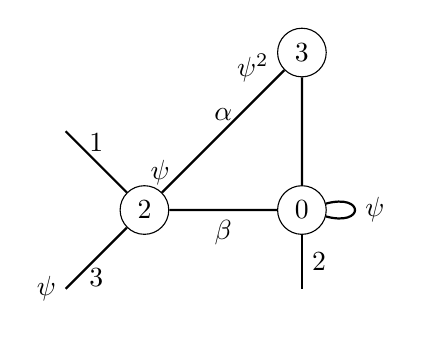
\begin{tikzpicture}[scale=1,transform shape,every loop/.style={}]
    \node[circle,draw] (A) at (0,0) {$2$};
    \node[circle,draw] (B) at (2,2) {$3$};
    \node[circle,draw] (C) at (2,0) {$0$};
    \draw[thick] (A) -- node[above]{$\alpha$} (B) -- (C) -- node[below]{$\beta$} (A);
    \draw[thick] (A) -- node[below]{$3$} (-1,-1);
    \draw[thick] (A) -- node[above]{$1$} (-1,1);
    \draw[thick] (C) -- node[right]{$2$} (2,-1);
    \draw[thick] (C) edge[loop right] node[right] {$\psi$} (C);
    \node[anchor=east] at (-1,-1) {$\psi$};
    \node[anchor=east] at (1.7,1.8) {$\psi^2$};
    \node[anchor=south] at (0.2,0.2) {$\psi$};
  \end{tikzpicture}
  \caption{Example of a stable graph in $\ol{\mc{M}}_{7,3}$ and associated tautological class. This stable graph describes the image of a map
    $\ol{\mc{M}}_{2,4} \times \ol{\mc{M}}_{3,2} \times \ol{\mc{M}}_{0,5} \to \ol{\mc{M}}_{7,3}$.}
  \label{fig:stablegraph}
\end{figure}

The first type of action on CohFTs is a translation action. Let $T \in V\ps{z}$. For a CohFT $\Omega$, we define
\[ (T\Omega)_{g,n}(\bv) \coloneqq \sum_m \frac{1}{m!} p_* \Omega_{g,n+m}(\bv, T,\ldots,T) \]
whenever the infinite sum makes sense.

\begin{exm}
    If $\Omega^X$ is the GW CohFT of a smooth projective variety $X$ and $\tau \in H^2(X)$ is a divisor class, then the infinite sum makes sense and we can define the shifted GW CohFT $\Omega^{X,\tau}$ of $X$. For example, if $X$ is the quintic threefold and $\tau = \frac{I_1}{I_0} H$, then shifting to $\tau$ is the same as the mirror map $q \mapsto Q(q) = q e^{\frac{I_1}{I_0}}$.
\end{exm}

The second type of action is the action of a matrix $R$ as in the beginning of this section. Let $G_{g,n}$ define the set of all stable graphs of genus $g$ with $n$ legs. Then we define
\[ (R\Omega)_{g,n} \coloneqq \sum_{\Gamma \in G_{g,n}} \frac{1}{\ab|\Aut \Gamma|} \on{Cont}_{\Gamma}, \]
where $\on{Cont}_{\Gamma}$ is defined by the following construction:
\begin{itemize}
    \item At the $i$-th leg, we place the map 
        \[ R(-\bar{\psi}_i)^* \in \Hom(V',V) \ps{\bar{\psi}_i}; \]
    \item At every edge, we place the bivector
        \[ V(\bar{\psi}_1, \bar{\psi}_2) \coloneqq \sum_{\mu} \frac{e_{\mu} \otimes e^{\mu} - R(-\bar{\psi}_1)^* e_{\mu} \otimes R(-\bar{\psi}_2)^* e^{\mu}}{\bar{\psi}_1 + \bar{\psi}_2}; \]
    \item At every vertex, we place the linear map
        \[ \Omega_{g_v, n_v} \colon V^{\otimes n_v} \to H^*(\Mbar_{g_v, n_v}); \]
    \item Finally, we consider the pushforward in cohomology along the gluing morphism $\prod_v \Mbar_{g_v, n_v} \to \Mbar_{g,n}$.
\end{itemize}

\begin{defn}
    Let $R$ be as above. Then we define the translation
    \[ T_R \coloneqq z (\1 - R(-z)^* \1') \in z V'\ps{z}. \]
    Whenever it makes sense, we define
    \[ R.\Omega \coloneqq RT\Omega. \]
\end{defn}

\begin{thm}[Chang-Guo-Li]
    Suppose we work with coefficients in $\C\ps{q}$. Then if
    \[ T_R \in z^2 V \ps{z} + zq V \ps{z}, \]
    $R.\Omega$ is a well-defined CohFT. Moreover, if $\dim V = \dim V'$, $\1'$ is a unit for $R.\Omega$.
\end{thm}

We would like to remark a bit more about the translation action when $R_0 \neq \mr{Id}$. For simplicity, we will assume that $V = V'$ and $R_0 \1 = c \cdot \1$ for some constant $c$. Then we set $\tilde{T}_R \coloneqq z( \1 - c R(z)^{-1} \1)$ and use the dilaton equation to compute
\begin{align*}
    T_R \Omega_{g,n}(\bv) &= \sum_{m=0}^{\infty} \frac{1}{m!} p_*\Omega_{g,n+m}(\bv, T_R, \ldots, T_R) \\
    &= \sum_{k,\ell \geq 0} \frac{1}{k!\ell!} p_* \Omega_{g,n+k+\ell}(\bv, ( (1-c^{-1})\1 \cdot \psi )^{\otimes k}, ( c^{-1} \tilde{T}_R )^{\otimes \ell}) \\
    &= \sum_{k,\ell \geq 0} \frac{(1-c^{-1})^k \cdot c^{-\ell}}{\ell!} \binom{2g-2+n+k+\ell-1}{k} p_* \Omega_{g,n+\ell}(\bv, \tilde{T}_R^{\otimes \ell}) \\
    &= \sum_{m=0}^{\infty} \frac{c^{2g-2+n}}{m!} p_* \Omega_{g,n+m}(\bv, \tilde{T}_R, \ldots, \tilde{T}_R)
\end{align*}
whenever this makes sense.


\subsection{Reconstruction theorem}%
\label{sub:Reconstruction theorem}

Recall that every CohFT defines a Frobenius algebra. We will call a CohFT \textit{semisimple} if the corresponding Frobenius algebra is semisimple.

\begin{thm}[Teleman]
    Let $\Omega$ be a semisimple CohFT with flat unit and $\omega$ be its topological part. If $\Omega$ is semisimple, there exists a unique 
    \[ R = \mr{Id} + R_1 z + \cdots \in \End(V)\ps{z} \]
    such that
    \[ \Omega = R.\omega. \]
\end{thm}

\begin{exm}
    Recall the Hodge bundle CohFT from before. Recall that it is given by the formula
    \[ \Omega^{\E}_{g,n} = c(\E) = 1 + \lambda_1 + \cdots + \lambda_g. \]
    Taking the degree zero part, we see that $\omega^{\E}$ is the GW CohFT of a point. Using Mumford's computation
    \[ \ch(\E) = g + \sum_{k=1}^{\infty} \frac{B_{2k}}{(2k)!}\ab(\kappa_{2k-1} + \frac{1}{2}\iota_*\sum_{i=0}^{2k-2} \bar{\psi}_1^{i} \bar{\psi}_2^{2g-2+i}), \]
    where $\kappa_{m} = p_* \bar{\psi}_{n+1}^{m+1}$, $B_{2k}$ are the Bernoulli numbers, and $\iota$ is the inclusion of the boundary up to a $2:1$ \'etale cover, and the formula
    \[ c(E) = \exp \ab(-\sum_k (-1)^k (k-1)!\ch_k(E)) \]
    for any vector bundle $E$ (or by just using the quantum Riemann-Roch theorem\footnote{There is a sign error in Coates-Givental, which has propagated to the rest of the literature.} directly), we obtain the $R$-matrix
    \[ R(z) = \exp\ab( \sum_{k=1}^{\infty} \frac{B_{2k}}{2k(2k-1)} z^{2k-1}) = 1+\frac{1}{12}z + \cdots. \]

    As a sanity check, we will compute $\Omega_{1,1}^{\E}$ using the $R$-matrix. First, we consider the stable graphs in~\Cref{fig:03graphloop}.
    \begin{figure}[htpb]
    \begin{center}
    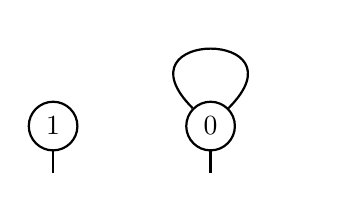
\begin{tikzpicture}[scale=1, transform shape, every loop/.style={}]
    \node[circle,draw=black,thick] (B) at (-1,0) {$1$};
    \draw[-,thick] (B) -- (-1,-0.6);
    \node[circle,draw=black,thick] (A) at (1,0) {$0$};
    \draw[-,thick] (A) -- (1,-0.6);
    \path[every node/.style={font=\sffamily\small},thick]
        (A)   edge[loop] (A);
    \end{tikzpicture}
    \end{center}
    \caption{Stable graphs for $g=1, n=1$}%
    \label{fig:03graphloop}
    \end{figure}
    The first graph $\Gamma_1$ gives us the contribution
    \begin{align*}
        \Cont_{\Gamma_1} &= T\omega_{1,1}^{\E}(R(z)^{-1}\1) \\
        &= \omega_{1,1}^{\E}(R(z)^{-1}\1) + p_* \omega_{1,1}^{\E}(R(z)^{-1}\1, T_R(z)).
    \end{align*}
    Using the formula $B_2 = \frac{1}{6}$ and the fact that $\dim \Mbar_{1,1} = 1$, this becomes
    \[ 1 - \frac{1}{12}\psi_1 + \frac{1}{12} \kappa_1. \]
    The second graph does not receive tail contributions because $\dim \Mbar_{0,3} = 0$. The constant term of the edge contribution is $\frac{1}{12}$, so considering the automorphism and pushing forward to $\Mbar_{1,1}$ gives us
    \[ \Cont_{\Gamma_2} = \frac{1}{12} \Delta, \]
    where $\Delta$ denotes the boundary divisor (with the correct stack structure). Because $\psi_1 = \kappa_1$ in this case, we obtain
    \[ 1+\lambda_1 = 1 + \frac{1}{12}(\kappa_1 - \psi_1 + \Delta) = 1 + \frac{1}{12} \Delta. \]
\end{exm}

\subsection{Operator formalism and geometric quantization}%
\label{sub:Operator formalism and geometric quantization}

We will return to the symplectic formalism of Givental. This is more convenient for certain computations, but it is in fact equal to what we have before, at least when we want to calculate generating functions. Recall that we had a Frobenius manifold structure on $V$ and we considered the vector space $\mc{V}\coloneqq V\ls{z^{-1}}$ with symplectic form
\[ (\mbf{f}(z), \mbf{g}(z)) \coloneqq \on{Res}_{z=0} \eta(\mbf{f}(-z), \mbf{g}(z)). \]
If we consider the polarization given by $\mc{V}_+ = V[z]$ and $\mc{V}_- = z^{-1}V\ps{z^{-1}}$, then letting $\bq$ be as before (with the dilaton shift), let $\bp$ be coordinates on $\mc{V}_-$ such that $(\bq, \bp)$ form a system of Darboux coordinates for $\mc{V}$.

\begin{defn}
    We will call any formal function of the form
    \[ \mc{D} = \exp\ab(\sum_{g=0}^{\infty} \hbar^{g-1} \mc{F}_g) \]
    an \textit{asymptotic element of the Fock space}.
\end{defn}

Then given such an asymptotic element of the Fock space, we will quantize (infinitesimal) symplectic transformations on $\mc{V}$ by the following formulae:
\[ \wh{p_a p_b} \coloneqq \hbar \partial_{q_a} \partial_{q_b}, \qquad \wh{p_a q_b} \coloneqq q_b \partial_{q_a}, \qquad \wh{q_a q_b} = \frac{q_a q_b}{\hbar}. \]
In particular, this will allow us to understand expressions like $\hat{R} \mc{D}$. However, we need to be careful because our formulae will involve both the fundamental solution $S_{\tau}$ and the $R$-matrix, and $S_{\tau}$ is a power series in $z^{-1}$.\footnote{This is because we expand $\frac{1}{z-\psi} = \sum_{n=0}^{\infty} \psi^n z^{-n-1}$.}

\begin{thm}[Givental]
    An operator of the form $S(z^{-1}) = \mr{Id} + S_1 z^{-1} + \cdots$ acts on (asymptotic) elements of the Fock space by the formula
    \[ \hat{S}^{-1} \mc{D}(\bq) = e^{\frac{1}{2\hbar}W(\bq,\bq)} \mc{D}([S \bq]_+), \]
    where $W = \sum \eta(W_{mn}q_m, q_n)$ is defined by the formula
    \[ \frac{S(w^{-1})^* S(z^{-1}) - \mr{Id}}{w^{-1}+z^{-1}} = \sum \frac{W_{mn}}{w^m z^n}. \]
    Operators of the form $R(z) = \mr{Id} + R_1 z + \cdots$ act by the formula
    \[ \hat{R}\mc{D}(\bq) = e^{\frac{\hbar}{2} V(\partial_{\bq}, \partial_{\bq})} \mc{D}(R^{-1} \bq), \]
    where $V = \sum \eta(p_m, V_{mn} p_n)$ is defined by 
    \[ \frac{R(w)^* R(z) - \mr{Id}}{w+z} = \sum V_{mn} w^m z^n. \]
\end{thm}

For a semisimple CohFT, there is a system of \textit{canonical coordinates} $u_{\alpha}$ such that the $1$-form $\d{u}$ is a homomorphism of algebras $T_v V \to \C$. Then near a semisimple point, there is a asymptotic solution to the quantum connection of the form
\[ \Psi \cdot  R \cdot e^{\frac{U}{z}}, \]
where $\Psi$ switches from flat coordinates to canonical coordinates and $U = \on{diag}(u_{\alpha})$ is the matrix of canonical coordinates. Finally, define
\[ C = \frac{1}{2} \int^u \sum R_1^{\alpha\alpha} \d{u_{\alpha}}. \]
A corollary of Teleman's reconstruction theorem is the formula
\[ \mc{D}^X = e^{C(u)} \hat{S}^{-1}_{\tau} \hat{\Psi} \hat{R} \wh{e^{\frac{U}{z}}} \prod_{i=1}^{\dim V} \mc{D}^{\mr{pt}} \]
for the Gromov-Witten theory of any smooth projective variety with semisimple quantum cohomology.

\begin{exm}
    As a final example, we will apply Teleman's theorem to compute $F_1$ of any semisimple CohFT. Let $e_{\mu}$ denote an idempotent basis for the quantum product. We will compute
    \[ \int_{\Mbar_{1,1}} \Omega_{1,1}(e_{\beta}). \]
    Using the reconstruction theorem, we obtain
    \begin{align*}
        \int_{\Mbar_{1,1}}\Omega_{1,1}(e_{\beta}) ={}& \int_{\Mbar_{1,1}} T_R \omega_{1,1}(R(\bar{\psi})^{-1} e_{\beta}) + \frac{1}{2} T_R \omega_{0,3}(R(\bar{\psi})^{-1} e_{\beta}, V(\bar{\psi}_2, \bar{\psi}_3)) \\
        ={}& \int_{\Mbar_{1,1}}T_R\omega_{1,1}(e_{\beta}) - \int_{\Mbar_{1,1}} T_R \omega_{1,1}(R_1 e_{\beta})\bar{\psi} \\ 
        &+ \frac{1}{2}\sum_{\mu}  \omega_{0,3}(e_{\beta}, R_1 e^{\mu}, e_{\mu}) \\
        ={}& \int_{\Mbar_{1,1}} ( \omega_{1,1}(e_{\beta}) + p_* ( \omega_{1,2}(e_{\beta}, R_1 \1) \bar{\psi}_2^2 )) \\
        &- \int_{\Mbar_{1,1}} (\omega_{1,1}(R_1 e_{\beta})\bar{\psi}_1 + p_* ( \omega_{1,2}(R_1 e_{\beta}) \bar{\psi}_2^2 ) \bar{\psi}_1) \\
        &+ \frac{1}{2} \sum_{\mu} \eta(e_{\beta} \star e_{\mu}, R_1 e^{\mu}) \\
        ={}& \frac{1}{24} \sum_{\mu} ( \omega_{0,4}(e_{\mu}, e^{\mu}, e_{\beta}, R_1 \1) -\omega_{0,3}(e_{\mu}, e^{\mu}, R_1 e_{\beta}) )\\
        &+ \frac{1}{2} \eta(e_{\beta}, R_1 e^{\beta}) \\
        ={}& \frac{1}{24} \sum_{\mu}\sum_{\nu} \omega_{0,3}(e_{\mu}, e^{\mu}, e_{\nu})\omega_{0,3}(e^{\nu}, e_{\beta}, R_1 \1) \\
        &-\frac{1}{24} \sum_{\mu} \omega_{0,3}(e_{\mu}, e^{\mu}, R_1 e_{\beta}) + \frac{1}{2} (R_1)_{\beta\beta} \\
        ={}& \frac{1}{24} \ab(\eta(e^{\beta}, R_1 \1) - \sum_{\mu} \eta(e^{\mu}, R_1 e_{\beta})) + \frac{1}{2} (R_1)_{\beta\beta}.
    \end{align*}
    Using the identities
    \begin{align*}
        \eta(R_1 \1, e^{\beta}) - \sum_{\mu} \eta(R_1 e_{\beta}, e^{\mu}) &= \sum_{\mu} \Delta_{\mu} \int_{\Mbar_{0,4}} \Omega_{0,4}(e_{\mu}, e_{\mu}, e_{\mu}, e_{\beta}) \\
        &= -\frac{1}{2}\sum_{\mu} \Delta_{\mu} \partial_{u_{\beta}} \Delta_{\mu}^{-1} \\
        &= \frac{1}{2} \sum_{\mu} \partial_{u_{\beta}} \log \Delta_{\mu},
    \end{align*}
    where $\Delta_{\mu} \coloneqq \eta(e_{\mu}, e_{\mu})^{-1}$, we obtain the result
    \[ \int_{\Mbar_{1,1}} \Omega_{1,1} e_{\beta} = \frac{1}{48} \sum_{\mu} \partial_{u_{\mu}} \log \Delta_{\mu} + \frac{1}{2} (R_1)_{\beta\beta}, \]
    which can be placed in the suggestive form
    \[ \d{F_1^{\Omega}} = \sum_{\mu} \frac{\d{\log \Delta_{\mu}}}{48} + \frac{1}{2} (R_1)_{\mu\mu} \d{u_{\alpha}}. \]
    This recovers a result which was already known to Givental.
\end{exm}

\part{Higher-genus computations via logarithmic GLSMs}
\label{pt:logglsm}

\section{Geometry of log GLSM moduli spaces (Qile Chen and Felix Janda)}%
\label{sec:Foundationslogglsm}

Our motivation is the quantum Lefschetz theorem. Here, we let $\mc{X}$ be a smooth projective variety or Deligne-Mumford stack over $\C$ and $E$ be a vector bundle over $\mc{X}$. We are interested in computing the Gromov-Witten invariants of a smooth complete intersection $\mc{Z} \subset \mc{X}$ defined by a regular section of $E$. Because the ambient space is generally easier to work with, it is desirable to find a way to compute the GW invariants of $\mc{Z}$ in terms of the data of $(\mc{X}, E)$.

\begin{quest}
    Is there a way to compute the Gromov-Witten invariants of $\mc{Z}$ using the ambient data of $(\mc{X}, E)$, possibly involving some correction terms?
\end{quest}

While quantum Lefschetz holds in genus zero in the convex case, and the approach of desingularization of the moduli of stable maps to force quantum Lefschetz to hold works well in genus one, this is intractable in higher-genus. Instead, our approach will be to use GLSMs, which were introduced by Witten in the physics literature, and by Fan-Jarvis-Ruan and Kiem-Li, Chang-Li, Chang-Li-Li, and other authors in mathematics. We will combine this with the theory of punctured log maps due to Abramovich-Chen-Gross-Siebert to obtain the theory of log GLSM.

\subsection{$R$-maps and log targets}%
\label{sub:R-maps}

\begin{defn}
    An \textit{$R$-map} is a commutative diagram
    \begin{equation*}
    \begin{tikzcd}
        & \mf{P} \ar{d} \\
        C \ar{d} \ar{ur}{f} \ar[swap]{r}{\omega_{\log}} & B \C^{\times}_{\omega} \\
        S,
    \end{tikzcd}
    \end{equation*}
    where the morphism $\mf{P} \to B\C_{\omega}^{\times}$ is a proper, log-smooth DM-type morphism. If the source is a twisted curve, this is the underlying $R$-map. If the source is a log curve, this is a \textit{log $R$-map}, and if the source is a punctured curve, this is a \textit{punctured $R$-map}.
\end{defn}

\begin{exm}
    Consider the diagram
    \begin{equation*}
    \begin{tikzcd}
        \mf{P}_{\C}^{\circ} = \on{Tot}(\mc{O}_{\P^n}(-d) \otimes \C_{\omega}) \ar{rr} \ar{d} & & \mf{P}^{\circ} = \on{Tot}(\mc{O}_{\P^n}(-d) \boxtimes \mc{L}_{\omega}) \ar{d} \\
        \Spec \C \ar{r} & B \C^{\times}_{\omega} & \P^n \times B \C_{\omega}^{\times} \ar{l}.
    \end{tikzcd}
    \end{equation*}
    Taking the base change of the underlying $R$-map to $C$, consider the diagram
    \begin{equation*}
    \begin{tikzcd}
        \mf{P}^{\circ} \times_{B \C_{\omega}^{\times}} C \ar{r} \ar{d} & \mf{P}^{\circ} \ar{d} \\
        C \ar{r} & B \C_{\omega}^{\times}.
    \end{tikzcd}
    \end{equation*}
    Therefore, the data of an $R$-map to this target is equivalent to the data of a morphism $C \to \P^n$ and a section $\rho \in H^0(f^* \mc{O}(-d) \otimes \omega_{\log})$. In particular, if $n=0$, we are left with the data of a differential $\rho \in H^0(\omega_{\log})$.
\end{exm}

\begin{exm}
    We will now give some examples of some log targets. An easy way to compactify a vector bundle is to turn it into a weighted projective space bundle, so for example we may consider
    \begin{equation*}
    \begin{tikzcd}
        \ul{\mf{P}}_{\ms{GW}, \C} = \P^{(\tilde{r},1)}(\mc{O}_{\P^n}(-d) \otimes \C_{\omega} \oplus \mc{O}) \ar{r} & \ul{\mf{P}}_{\ms{GW}} = \P^{(\tilde{r}, 1)}(\mc{O}_{\P^n}(-d) \oplus \mc{O}).
    \end{tikzcd}
    \end{equation*}
    We can give this the log structure of functions which vanish only on the boundary and call it $\mf{P}_{\GW}$.

    Another example is to consider the example of $5$-spin curves. Here, $\mc{X} = B \G_m$ with the degree $5$ map to $B \C_{\omega}^{\times}$. Then we set
    \[ \ul{\mf{P}}_{\mr{LG}} = \P(\mc{L}_{\mc{X}}^5 \oplus \mc{O}). \]
    Again, we give this the divisorial log structure and call it $\mf{P}_{\LG}$.

    A feature of this is that there is a geometric LG/CY correspondence, namely that $\infty_{\LG} \simeq \infty_{\GW}$ as log stacks.
\end{exm}

\begin{exm}
    For the $(3,3)$ complete intersection in $\P^5$, we consider
    \[ \mf{P}_{\GW} = \P(\mc{O}_{\P^5}(-3)^{\oplus 2} \otimes \mc{L}_{\omega} \oplus \mc{O}) \]
    with the divisorial log structure.
\end{exm}

\begin{exm}
    We will now consider a general hybrid target. The input is a smooth projective DM stack $X$, a vector bundle $E = \bigoplus E_i$ over $X$, a line bundle $L$ over $X$, and $r \in \Z_{>0}$. The spin is the diagram
    \begin{equation*}
    \begin{tikzcd}
        \mc{X} \ar{r}{\mc{L}_{\mc{X}}} \ar{d} & B \G_m \ar{d}{r} \\
        X \times B \C_{\omega}^{\times} \ar{r}{L^{-1} \otimes \mc{L}_{\omega}} & B \G_m
    \end{tikzcd}
    \end{equation*}
    The target is
    \[ \P\ab(\bigoplus E_i^{\vee} \otimes \mc{L}_{\mc{X}}^i \oplus \mc{O}) \]
    with the divisorial log structure at infinity.
\end{exm}

We will now turn our discussion to the discrete data. This consists of a genus, curve class, and twisted sector for each marking. We will now construct a dual graph, which has vertices and half-edges. There is an involution 
\[\iota_G \colon V \cup H \to V \cup H \]
and a vertex map $v_G \colon H \to V$. Legs are the half-edges which are fixed by the involution, and we will label the legs by the marking map
\[ m \colon L \to \{1,\ldots,n\}. \]
The decorations are the curve classes, sectors, and degrees.

Consider a log map
\begin{equation*}
\begin{tikzcd}
    & \mf{P} \ar{d} \\
    P_h \subset C \ar{ur}{f} \ar{r}_{\omega_{\log}} & B \C_{\omega}^{\times},
\end{tikzcd}
\end{equation*}
where $P_h$ is a special point. Because $\omega_{\log}|_{P_h}$ is the trivial bundle, we obtain a commutative diagram
\begin{equation*}
\begin{tikzcd}
    P_h \ar{r} \ar{d} & \mf{P}_{\C} \ar{d} \\
    C \ar{r}{f} & \mf{P},
\end{tikzcd}
\end{equation*}
which exhibits $P_h$ as a gerbe over $\mf{P}_{\C}$. Assuming that there are no orbifold points, theere is a sector map
\[ \ol{r} \colon H(G) \to \ab\{ 0_{\mf{P}_{\C}}, \infty_{\mf{P}_{\C}}, \mf{P}_{\C}\}. \]
We require that $P_h \to \mf{P}_{\C}$ factors through $\ol{r}_h$, and say that $h$ is \textit{compact type} if $\ol{r}_h = 0_{\mf{P}}$.

\begin{exm}
    Consider again $X = \P^0$. Then $\mf{P} = \P(\mc{L}_{\omega} \oplus \mc{O})$. If $g=1$, then a log map is simply $\eta \in H^0(\omega_C)$, which cannot be stable. Adding a marked point, we obtain a section of $\omega_C^{\log}$, which we will force to vanish at the marked point.
\end{exm}

The stability of underlying $R$-maps has two conditions:
\begin{enumerate}
    \item First, that the morphism is representable;
    \item Second, that
        \[ (\omega_{\log})^{1+\delta} \otimes f^* H^{\otimes k} \otimes f^* \mc{O}(\tilde{r}\infty) > 0, \]
        where $H$ is a polarization on the target. Here, $k \gg 1 \gg \delta > 0$.
\end{enumerate}

\begin{exm}
    Again considering $X = \P^0$, we will let $C$ be of genus $2$. the limit $\lim_{\lambda \to \infty} \lambda \cdot \eta$ is the union of a genus-zero curve with a differential which vanishes at one point with multiplicity $2$ connected to a genus $2$ curve which sits entirely at infinity. Even though the rational component is not a priori stable, it is stabilized by its intersection with the zero section.
\end{exm}

\begin{rmk}
    In the $\P^0$ case, stability is equivalent to the condition that
    \[ \omega^{\log} \otimes \eta^* \mc{O}(k \cdot 0_{\mf{P}}) > 0 \]
    whenever $k \gg 1$.
\end{rmk}

\subsection{Log geometry and tropicalization}%
\label{sub:Log geometry and tropicalization}


\begin{defn}
    Let $\ul{Y}$ be a scheme or a stack. A \textit{log structure} on $\ul{Y}$ is a sheaf of monoids $\mc{M}_Y$ on $\ul{Y}$, together with a morphism
    \[ \alpha \colon \mc{M}_Y \to (\mc{O}_{\ul{Y}}, \cdot) \]
    inducing an isomorphism $\alpha^{-1} \mc{O}_{\ul{Y}}^{\times} \simeq \mc{O}_{\ul{Y}}^{\times}$. The pair $Y = (\ul{Y}, \mc{M}_Y)$ is called a \textit{log scheme/stack} and the sheaf
    \[ \ol{\mc{M}}_{Y}/\mc{O}_{\ul{Y}}^{\times} \]
    is called the \textit{characteristic sheaf} or \textit{ghost sheaf}.
\end{defn}

\begin{exm}
    Any log GLSM target is a log stack.
\end{exm}

\begin{exm}
    Another standard target is a toric variety with $\mc{M}_Y$ being all functions which vanish only on the toric boundary. This is usually called the divisorial log structure.
\end{exm}

\begin{exm}
    For a toric monoid $P$, we can consider
    \[ S = \Spec(P \to \C) = (\Spec \C, P \times \mc{O}_{\Spec \C}^{\times}). \]
\end{exm}

The tropical data we will consider is the category $\ms{Cones}$ of rational polyhedral cones $(\sigma, N)$. This has a distinguished object $(\R_{\geq 0, \Z})$. Locally, we will define
\[ \Sigma(\Spec (P \to \C)) = \Hom(P, R_{\geq 0}) = P_{\R}^{\vee} \]
with the natural lattice structure $P^{\vee} \coloneqq \Hom(P, \N)$. In general, the tropicalization $\Sigma(X)$ of a log scheme $X$ is the generalized cone complex given by gluing local pictures along face maps.

\begin{exm}
    Consider $\A^1$ with the log structure given by $0$. Then
    \[ \Sigma(\A^1) = \R_{\geq 0}. \]
    Here, there is only a log structure at $0$, which is a copy of $\N$ measuring the vanishing order at the origin. The map
    \[ \ol{M}_{\A^1, 0} \to \ol{M}_{\A^1, x} \]
    sends $1$ to $0$, so induces $0 \hookrightarrow \N^{\vee}$.
\end{exm}

\begin{exm}
    Consider $\A^2$ with the toric log structure. Then $\Sigma(\A^2)$ is simply $\R_{\geq 0}^2$, which is the same as the support of the toric fan. At the monoid level, there is an $\N^2$ at the origin, a copy of $\N$ on each axis, and $0$ at a general point.
\end{exm}

\subsection{Log curves}%
\label{sub:Log curves}

\begin{defn}
    An \textit{$n$-pointed log curve} over a log scheme $S$ consists of
    \[ (\pi \colon C \to S, \{p_i\}_{i=1}^n ), \]
    such that
    \begin{enumerate}
        \item The underlying morphism of $\pi$ is an $n$-pointed twisted curve;
        \item $\pi$ is log smooth and integral;
        \item On the smooth locus of $C$, the log structure is given by $\ol{M}_S \oplus \bigoplus_{i=1}^n \N \cdot p_i$
    \end{enumerate}
\end{defn}

Intuitively, the log structure is given by the log structure $\ol{M}_S$ at smooth unmarked points, $\ol{M}_S \oplus \N$ at marked points, and $\ol{M}_S \oplus_{\N} \N^2$ at the nodes, which means the pushout diagram
\begin{equation*}
\begin{tikzcd}
    \N \ar{r}{\Delta} \ar{d}{\ell} & \N^2 \ar{d} \\
    \ol{M}_S \ar{r} & \ol{M}_C|_q.
\end{tikzcd}
\end{equation*}
Here, $\ell$ is the edge length parameter, and $(1,0)$ and $(0,1)$ are the two components.

Because tropicalization is functorial, the morphism $C \to S$ induces a morphism
\[ \Sigma(C) \to \Sigma(S). \]
For example, if $C$ has two components, then the node will correspond to the largest cone, each component corresponds to a copy of $\ol{M}_S$, and each marking will give a leg of infinite length. Above a point in $\Sigma(S)$, the distance between the two components is the edge length parameter evaluated at the point $x$. To see this more clearly, see~\Cref{fig:tropcurve-png}.
\begin{figure}[htpb]
    \centering
    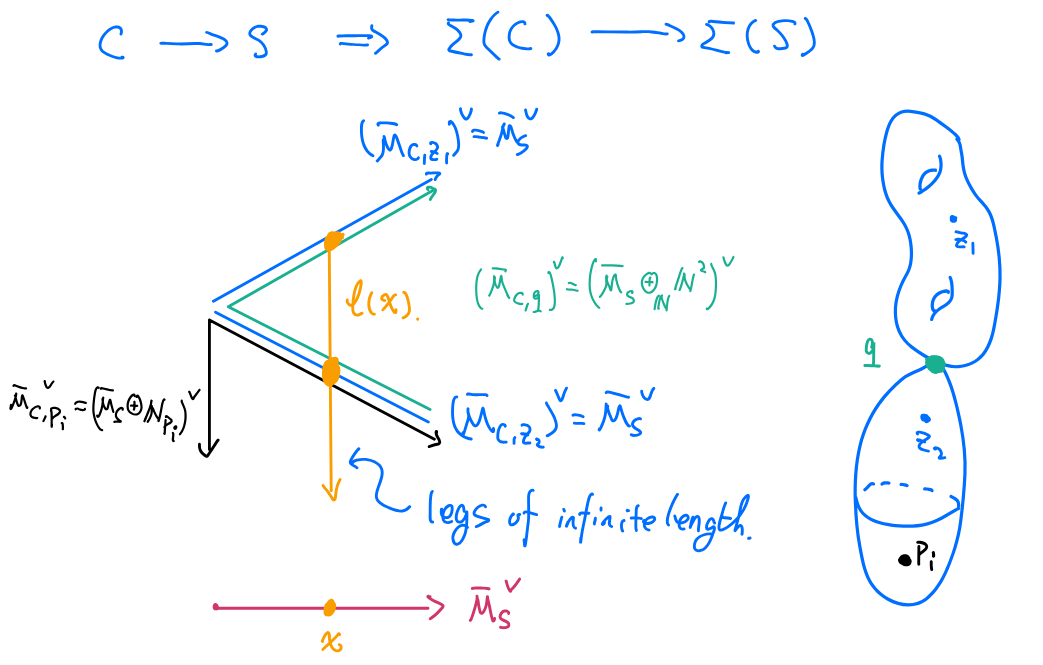
\includegraphics[width=0.8\textwidth]{tropcurve.png}
    \caption{Tropicalization of a log curve.}
    \label{fig:tropcurve-png}
\end{figure}

We will now consider punctured curves. We will consider a diagram
\begin{equation*}
\begin{tikzcd}
    p_i^{\circ} \ar{r} \ar{d} & p_i \ar{d} \\
    C^{\circ} \ar{r}{P} & C \ar{r} & S.
\end{tikzcd}
\end{equation*}
Here, $P$ is a morphism of log schemes which is an isomorphism away from $P_i$ and $\ul{P}$ is an isomorphism. In addition, we will have an inclusion
\[ \ol{M}_{C,p_i} = \ol{M}_S \oplus \N p_i \subset \ol{M}_{C^{\circ}, p_i} = \ol{M}_S \oplus \Z p_i. \]
This corresponds to allowing poles at $p_i$, and in the tropicalization makes edges finite-length. A picture is given in~\Cref{fig:punctured-png}.
\begin{figure}[htpb]
    \centering
    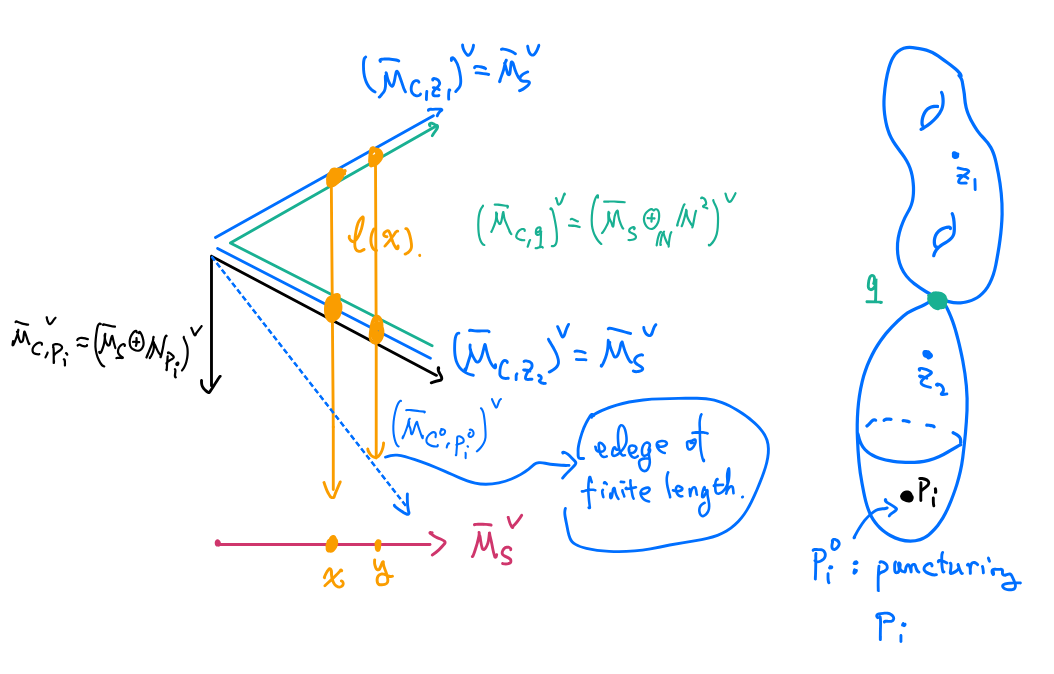
\includegraphics[width=0.8\textwidth]{punctured.png}
    \caption{Tropicalization of a punctured curve.}
    \label{fig:punctured-png}
\end{figure}

\begin{defn}
    A \textit{punctured curve} is a log curve with punctures
    \[ \C^{\circ} \to C \to S. \]
    A \textit{tropical punctured curve} is a tropical curve with the additional data of lengths of punctured legs.
\end{defn}

\subsection{Superpotentials}%
\label{sub:Superpotentials}

\begin{defn}
    A \textit{superpotential} is a commutative diagram
    \begin{equation*}
    \begin{tikzcd}
        \mf{P}^{\circ} \ar{r} \ar{dr} & \mc{L}_{\omega} \ar{d} \\
        & B \C^{\times}_{\omega},
    \end{tikzcd}
    \end{equation*}
    where $\mf{P}^{\circ} = \mf{P} \setminus \infty$. We say that $W$ has \textit{proper critical locus} if
    \[ \on{Crit} W \to B \C_{\omega}^{\times} \]
    is proper.
\end{defn}

Equivalently, a superpotential is a $\C_{\omega}^{\times}$-equivariant function
\[ W_{\C} \colon \mf{P}_{\C}^{\circ} \to \C_{\omega}. \]
In this formulation, $W$ has proper critical locus if and only if $\on{Crit} W_{\C}$ is proper (as a DM stack). This implies that the critical locus is contained in $0_{\mf{P}}$.

\begin{exm}
    Let $X$ be a smooth projective Deligne-Mumford stack and $E$ be a vector bundle on $X$ with section $s$. We will write
    \[ W_{\C} = \otimes (s \otimes 1_{\C_{\omega}}) \colon \mf{P}_{\C}^{\circ} = E^{\vee} \otimes \C_{\omega} \to \C_{\omega}. \]
    Then $\Crit W_{\C}$ is proper if and only if $Z = (s=0)$ is smooth of codimension equal to the rank of $E$.
\end{exm}

\begin{exm}
    Let $X = \P^0$ and $E = \C$. Let $s \in H^0(E)$ be nonzero. Now $W_{\C}$ is simply multiplication by $s$, so the critical locus is empty.
\end{exm}

\subsection{Punctured $R$-maps}%
\label{sub:Punctured R-maps}

\begin{defn}
    A \textit{punctured $R$-map} is an $R$-map with domain a punctured $R$-map.
\end{defn}

\begin{defn}
    Let $h$ be a half-edge. Then the \textit{contact order} at $h$ is defined by
    \[ c(h) \coloneqq \pdv{\on{Trop} f}{u_h} \in \Z. \]
\end{defn}

\begin{figure}[htpb]
    \centering
    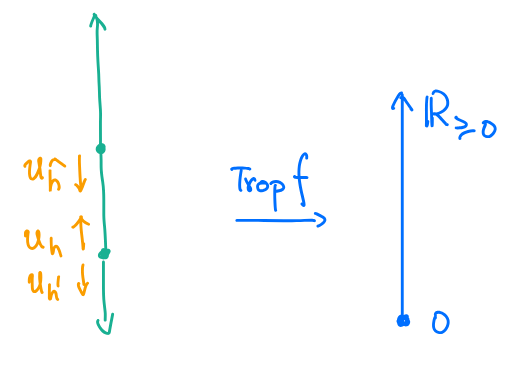
\includegraphics[width=0.5\textwidth]{interval.png}
    \caption{Contact orders. Note the last downward edge has finite length.}
    \label{fig:interval-png}
\end{figure}


\begin{exm}
    Consider the genus $2$ picture from before (target being $\P^0$) and consider the same stable limit as an $R$-map. If we calculate with $z = s^{-1}$, then
    \[ z^2 \d{z} = -s^{-3} \frac{\d{s}}{s}, \]
    so the pole order at the node must be $3$. Tropically, if $\hat{h}$ is the half edge of the node attached to the $g=2$ vertex, we have $c(\hat{h}) = -3$, so restricting to the $g=2$ component, we obtain a punctured $R$-map.
\end{exm}

The discrete data of punctured $R$-maps is
\[ \bm{\tau} = (G, g, \beta, \deg, \ol{r}, \sigma\colon V \cup H \to \{0,R_{\geq 0}\}, c \colon H \to \Z). \]

\begin{thm}
    The moduli stack $\mc{R}(\mf{P}, \bm{\tau})$ is a proper log DM stack admitting a canonical perfect obstruction theory.
\end{thm}


\begin{defn}
    We will consider $\bm{\tau}$ where $V(G) = \{\star\}$ and $L(G) = H(G)$. These are called \textit{vertex-type moduli}. If $\sigma = 0$, then we will denote
    \[ \mc{R}_{g,\mc{C}}(\mf{P}, \beta) \coloneqq \mc{R}(\mf{P}, \bm{\tau}) \]
    for the stack of stable log $R$-maps,
    and if $\sigma = \R_{\geq 0}$, the we will denote
    \[ \mc{R}_{g,\mc{C}}(\infty, \beta) \coloneqq \mc{R}(\mf{P}, \btau) \]
    for the stack of punctured $R$-maps.
\end{defn}

\subsection{Obstruction theories}%
\label{sub:The canonical perfect obstruction theory}


\begin{defn}
    Recall that we have a diagram
    \begin{equation*}
    \begin{tikzcd}
        & \mf{P} \ar{d} \\
        C \ar{r} \ar{d}{\pi} \ar{ur}{f} & B \C_{\omega}^{\times} \\
        \mc{R}(\mf{P}, \btau).
    \end{tikzcd}
    \end{equation*}
    The \textit{canonical perfect obstruction theory} is defined by
    \[ \varphi \colon \mathbb{T}_{\mc{R}(\mf{P}, \beta)/\mf{M}(\btau)} \to R \pi_* f^* T_{\mf{P}/B\C_{\omega}^{\times}}. \]
    Because it is very complicated, we will not discuss $\mf{M}(\btau)$.
\end{defn}


Unfortunately, this is not the obstruction theory that we really want. We will consider the superpotential and then use the cosection localization technique of Kiem-Li. Here, we have the diagram
\begin{equation*}
\begin{tikzcd}
    & \mf{P}^{\circ} \ar{r}{W} \ar{d} & \mc{L}_{\omega} \ar{dl} \\
    C \ar[swap]{r}{\omega_{\log}} \ar{d}{\pi} & B \C_{\omega}^{\times} \\
    S
\end{tikzcd}
\end{equation*}
whenever $\btau$ is of compact type. The compact-type condition implies that
\[ f^* \d{W} \colon f^* T_{\mf{P}^{\circ}/B\C_{\omega}^{\times}} \to \omega_{\log} \]
factors through the sheaf $\omega$ of holomorphic differentials. Because $R^1 \pi_* \omega \cong \mc{O}$, we obtain a cosection
\[ \sigma_W \coloneqq R^1 \pi_* f^* \d{W} \colon R^1 \pi_* f^* T_{\mf{P}^{\circ}/B \C_{\omega}^{\times}} \to \mc{O}. \]
By the results of Kiem-Li, this gives us a virtual cycle
\[ [\mc{R}_{g, \mc{C}}(\mf{P}^{\circ}, \beta)]^{\vir}_{\sigma_W} \]
supported on $R$-maps to $\Crit W$,
which coincides with the canonical virtual cycle after pushing forward to the stack of all $R$-maps.

\begin{rmk}
    In Gromov-Witten theory, the cosection localized virtual cycle satisfies the relation
    \[ [ \mc{R}_{g, \mc{C}}(\mf{P}^{\circ},\beta) ]^{\vir}_{\sigma_W} = \pm [\Mbar_{g,n}(Z,\beta)]^{\vir} \]
    by work of Chang-Li, Chang-Li, Kim-Oh, Picciotto, and Chen-Janda-Webb.
\end{rmk}

Of course, we have the problem that $\mc{R}_{g, \mc{C}}(\mf{P}^{\circ}, \beta)$ is not proper, so we need to find a way to extend the cosection along the boundary
\[ \Delta_{g, \mc{C}} (\mf{P}, \beta) \coloneqq \mc{R}_{g, \mc{C}}(\mf{P}, \beta) \setminus \mc{R}_{g,\mc{C}}(\mf{P}^{\circ}, \beta). \]
We need to understand how to differentiate
\[ W \colon \mf{P} \dashrightarrow \mc{L}_{\omega}, \]
which will require compact-type legs and a principalization of the boundary.

\begin{defn}
    We will say discrete data is \textit{compact type} if for all $h \in L(G)$, either
    \begin{itemize}
        \item $c(h) = 0$ and $\bar{r} = 0_{\mf{P}}$;
        \item $c(h) \leq -1$. In this case $\bar{r} = \infty_{\mf{P}}$.
    \end{itemize}
\end{defn}

\begin{exm}
    Consider the $\P^0$ example in genus $1$. If we consider $\eta \in H^0(\omega_C)$, we can view it as $\eta \in H^0(\omega_C^{\log})$. Then, at the marking, we see that $c(h) = 0$ and $\bar{r}_h = 0_{\mf{P}}$, so the leg is of compact type. In the tropical picture, the entire infinite leg gets contracted to the origin.
\end{exm}

\begin{exm}
    Now consider the same example but with $g=2$. We will impose that there are no markings by $(\eta = 0) = 2p$. The stable limit as we scale $\eta$ to infinity had a genus $0$ component with a zero of order $2$ and a genus $2$ component mapping entirely to $\infty$. If we consider the half-edge emerging from the genus $0$ vertex, it touches $\infty$ with contact order $3$, so it is not compact type. On the other hand, the half-edge coming from the genus $2$ vertex touches $\infty$ with contact order $-3$, so it is compact type (and in the tropical picture the leg has finite length).

    \begin{rmk}
        The data of $\eta_0 |_{C_2}$ is equivalent to a fixed isomorphism $\mc{O}_{C_2}(2p) \simeq \omega_{C_2}$, where $C_2$ is the genus $2$ vertex.
    \end{rmk}
\end{exm}

\begin{rmk}
    Tropical curves with only compact-type legs have compact image in $\Sigma(\mf{P}) = \R_{\geq 0}$. In this picture, they are either pointing downward or contracted to the origin.
\end{rmk}

Having defined compact type insertions, we will now define a modular principalization of the boundary. There is an edge length
\[ \ell \colon E(G) \cup L^{\circ}(G) \to \ol{M}_S \]
and a degeneracy
\[ e \colon V(G) \to \ol{M}_S \]
which intuitively records where $v$ is sent in $\R_{\geq 0}$.

\begin{defn}
    For a toric monoid $P$, define a partial order $a \leq b$ if there exists $c \in P$ such that $a+c = b$. If we consider a punctured $R$-map, consider the collection of degeneracies
    \[ \{ e_V \mid v \in V(G)\}. \]
    It has \textit{uniform maximal degeneracy} if there is a unique maximum
    \[ e_{\max} = \max \{e_v \mid v \in V(G)\}. \]
\end{defn}

\begin{exm}
    Let $\ol{M}_S = \N^2$. Suppose that there are $v_1, v_2$ and a vertex $v_0$ which is sent to $0 \in \R_{\geq 0}$. Then we compute
    \begin{align*}
        e_{v_1} &= e_{v_0} + c_1 \cdot \ell_1 \\
        &= \ell_1.
    \end{align*}
    Similarly, $e_{v_2} = \ell_2$, where $\ell_1$ and $\ell_2$ are the generators of $\N^2$. These cannot be compared, so we do not have uniform maximal degeneracy.

    To uniformize this, we consider a subdivision into three subcones. The first is when $\ell_2 > \ell_1$, the second is when $\ell_1 = \ell_2$, and the third is when $\ell_1 > \ell_2$. After this subdivision, each subcone has uniform maximal degeneracy.
\end{exm}

\begin{exm}
    A family of tropical curves over $\bar{M}_S^{\vee}$ with compact-type legs and uniform maximal degeneracy $e_{\max} \in \ol{M}_S$ has images in $\R_{\geq 0}$ uniformly bounded from above by $e_{\max}$.
\end{exm}

We now define a new stack
\[ \mc{U}(\mf{P}, \btau) \]
to be the stack of punctured $R$-maps with discrete data $\btau$ and having uniform maximal degeneracy. By removing the condition of uniform maximal degeneracy, we obtain a morphism
\[ F \colon \mc{U}(\mf{P}, \btau) \to \mc{R}(\mf{P}, \btau), \]
which satisfies the following:
\begin{itemize}
    \item $F$ is log \'etale, proper, and surjective;
    \item There is as canonical perfect obstruction theory;
    \item We have
        \begin{align*}
            F_* [ \mc{U}_{g, \mc{C}}(\mf{P}, \beta) ]^{\vir} &= [\mc{R}_{g,\mc{C}}(\mf{P}, \beta) ]^{\vir}_{\sigma_W} \\
            F_* [ \mc{U}_{g, \mc{C}}(\mf{P}, \beta) ]^{\vir} &= [\mc{R}_{g,\mc{C}}(\infty, \beta) ]^{\vir}_{\sigma_W}
        \end{align*}
        for vertex-type moduli.
\end{itemize}

The boundary $\Delta_{g, \mc{C}}(\mf{P}, \beta)^{\curlywedge}$ defined by the Cartesian diagram
\begin{equation*}
\begin{tikzcd}
    \Delta^{\curlywedge} \ar{r} \ar{d} & \Delta_{\max} = 0 \ar{d} \\
    \mc{U} \ar{r} & { [\A^1/\G_m] }
\end{tikzcd}
\end{equation*}
is a log Cartier divisor.

\begin{thm}
    Assume all legs are of compact type and $W \colon \mf{P}^{\circ} \to \mc{L}_{\omega}$ has proper critical locus. Then
    \begin{enumerate}
        \item $\mc{U}(\mf{P},\btau)$ has a reduced perfect obstruction theory;
        \item In the log $R$-map case, we have
            \[ [\mc{U}_{g, \mc{C}}(\mf{P},\beta)]^{\on{red}} = [\mc{R}_{g,\mc{C}}(\mf{P}^{\circ}, \beta)]^{\vir}_{\sigma_W}; \]
        \item The boundary $\Delta_{g, \mc{C}}^{\curlywedge}(\mf{P}, \beta)$ also has a reduced perfect obstruction theory;
        \item There is the relation
            \[ [\mc{U}_{g, \mc{C}}(\mf{P}, \beta)]^{\on{red}} = [\mc{U}_{g, \mc{C}}(\mf{P}, \beta)]^{\vir} - \tilde{r} [\Delta^{\curlywedge}_{g, \mc{C}}(\mf{P}, \beta)]^{\on{red}}, \]
            where $\tilde{r}$ is the pole order of $W$ at infinity.
    \end{enumerate}
\end{thm}

The reduced perfect obstruction theory for log $R$-maps is given by the triangle
\[ \E^{\on{red}} \to R \pi_* f^* T_{\mf{P}/B\C_{\omega}^{\times}} \xrightarrow{\sigma} [\mc{O} \to \mc{O}(\tilde{r}\Delta_{\max})] \xrightarrow{[1]} \]
and for $e_{\max} > 0$ is given by
\[ \E^{\on{red}} \to R \pi_* f^* T_{\mf{P}/B\C_{\omega}^{\times}} \xrightarrow{\sigma} \mc{O}(\tilde{r})[-1] \xrightarrow{[1]}. \]

The virtual components of $\Delta_{g,\mc{C}}^{\curlywedge}$ are given by the formula
\[ [\Delta_{g, \mc{C}}^{\curlywedge}(\mf{P}, \beta)]^{\on{red}} = \sum_{\btau_{\curlywedge}} \frac{\on{lcm}_{x\in E(G)} c(x)}{\ab|\Aut \btau_{\curlywedge}|} [\mc{U}(\mf{P}, \btau_{\curlywedge})]^{\on{red}} \]
due to Abramovich-Chen-Gross-Siebert, where
\[ \btau_{\curlywedge} = (\btau, V_{\max}(G)) \]
is the tropical type of rigid tropical curves with uniform maximal degeneracy. Here, this implies that $\btau_{\curlywedge}$ is bipartite and rigidity means there is no deformation fixing $\btau$ and $V_{\max}(G)$ besides scaling $e_{\max}$

Decomposing this further, we have
\begin{align*}
    &[\mc{U}(\mf{P}, \btau_{\curlywedge})]^{\on{red}} \\ 
    &= (-\tilde{r})^{|V_{\infty}(G)|-1} \frac{\prod_{E \in E(G)} c(E)}{\on{lcm}_{E \in E(G)} c(E)} \Delta^!_{\btau_{\curlywedge}} \ab(\prod_{v \in V_{\infty(G)}} [\mc{U}(\mf{P}, \btau_v)]^{\on{red}} \times \prod_{v \in V_0(G)} [\mc{U}(\mf{P}, \btau_V)]^{\vir}). 
\end{align*}
This is not true if we replace everything with the canonical obstruction theory, so this is quite interesting. Putting these two formulae together, we obtain the tropical decomposition formula
\begin{align*}
    [\mc{U}_{g, \mc{C}}(\mf{P}, \beta)]^{\on{red}} = \sum_{\btau_{\curlywedge}} & \frac{(-\tilde{r})^{|V_{\infty}(G)|}}{|\Aut \btau_{\curlywedge}|} \cdot \prod_{E \in E(G)} c(E) \cdot \\
    & \cdot \Delta_{\btau_{\curlywedge}}^! \ab( \prod_{v \in V_{\infty}(G)}[\mc{U}(\mf{P},\btau_{v})]^{\red} \times \prod_{v \in V_0(G)} [\mc{U}(\mf{P},\btau_v)]^{\vir}).
\end{align*}

\begin{exm}
    Consider the $\P^0$ example again. When $g=2$, we obtain six bipartite graphs, which are given in~\Cref{fig:tropgraphs}.
    \begin{figure}[htpb]
    \begin{center}
    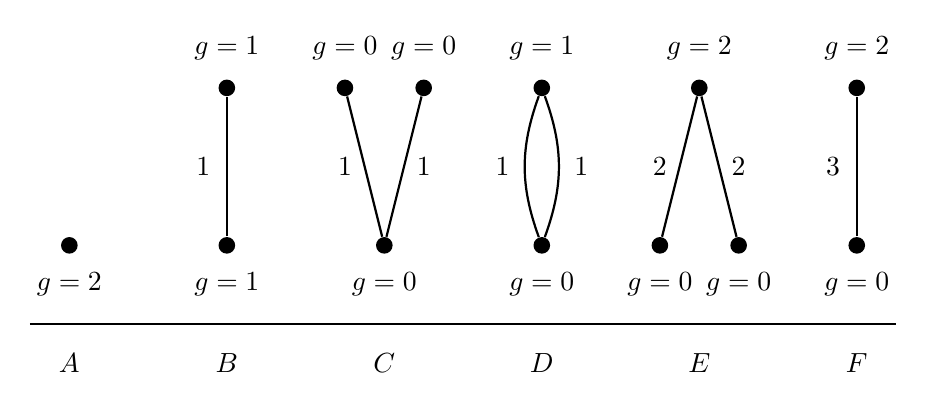
\begin{tikzpicture}[scale=1, transform shape]
        \node[fill=black,circle,minimum size=6pt,inner sep=0pt] (A) at (0,0) {};
        \node[fill=black,circle,minimum size=6pt,inner sep=0pt] (B1) at (2,0) {};
        \node[fill=black,circle,minimum size=6pt,inner sep=0pt] (B2) at (2,2) {};
        \node[fill=black,circle,minimum size=6pt,inner sep=0pt] (C1) at (4,0) {};
        \node[fill=black,circle,minimum size=6pt,inner sep=0pt] (C2) at (3.5,2) {};
        \node[fill=black,circle,minimum size=6pt,inner sep=0pt] (C3) at (4.5,2) {};
        \node[fill=black,circle,minimum size=6pt,inner sep=0pt] (D1) at (6,0) {};
        \node[fill=black,circle,minimum size=6pt,inner sep=0pt] (D2) at (6,2) {};
        \node[fill=black,circle,minimum size=6pt,inner sep=0pt] (E1) at (8,2) {};
        \node[fill=black,circle,minimum size=6pt,inner sep=0pt] (E2) at (7.5,0) {};
        \node[fill=black,circle,minimum size=6pt,inner sep=0pt] (E3) at (8.5,0) {};
        \node[fill=black,circle,minimum size=6pt,inner sep=0pt] (F1) at (10,0) {};
        \node[fill=black,circle,minimum size=6pt,inner sep=0pt] (F2) at (10,2) {};
        \draw[-,thick] (B1) -- (B2);
        \draw[-,thick] (C2) -- (C1) -- (C3);
        \draw[-,thick] (D1) edge[bend left=20] (D2);
        \draw[-,thick] (D2) edge[bend left=20] (D1);
        \draw[-,thick] (E2) -- (E1) -- (E3);
        \draw[-,thick] (F1) -- (F2);
        \node at (0,-0.5) {$g=2$};
        \node at (2,-0.5) {$g=1$};
        \node at (4,-0.5) {$g=0$};
        \node at (6,-0.5) {$g=0$};
        \node at (7.5,-0.5) {$g=0$};
        \node at (8.5,-0.5) {$g=0$};
        \node at (10,-0.5) {$g=0$};
        \node at (2,2.5) {$g=1$};
        \node at (3.5,2.5) {$g=0$};
        \node at (4.5,2.5) {$g=0$};
        \node at (6,2.5) {$g=1$};
        \node at (8,2.5) {$g=2$};
        \node at (10,2.5) {$g=2$};
        \draw[-,thick] (-0.5,-1) -- (10.5,-1);
        \node at (0,-1.5) {$A$};
        \node at (2,-1.5) {$B$};
        \node at (4,-1.5) {$C$};
        \node at (6,-1.5) {$D$};
        \node at (8,-1.5) {$E$};
        \node at (10,-1.5) {$F$};
        \node at (1.7,1) {$1$};
        \node at (3.5,1) {$1$};
        \node at (4.5,1) {$1$};
        \node at (5.5,1) {$1$};
        \node at (6.5,1) {$1$};
        \node at (7.5,1) {$2$};
        \node at (8.5,1) {$2$};
        \node at (9.7,1) {$3$};
    \end{tikzpicture}
    \end{center}
    \caption{Graphs of tropical types for $X = \P^0$ when $g=2$.}%
    \label{fig:tropgraphs}
    \end{figure}
    Choosing any nonzero superpotential, we obtain the tropical decomposition formula
    \begin{align*}
        0 ={}& [\mc{U}_g(\mf{P},0)]^{\red} = \sum_{\btau_{\curlywedge}} \frac{(-1)^{|V_{\infty}(G)|}} \cdot \prod_{E \in E(G)} c(E) \\
    & \cdot \Delta_{\btau_{\curlywedge}}^! \ab( \prod_{v \in V_{\infty}(G)}[\mc{U}(\mf{P},\btau_{v})]^{\red} \times \prod_{v \in V_0(G)} [\mc{U}(\mf{P},\btau_v)]^{\vir}).
    \end{align*}
    Note here that the critical locus is empty, so the virtual cycle must be zero.
\end{exm}


In GW theory, the tropical decomposition formula becomes
\begin{align*}
    [\Mbar_{g,n}(Z,\beta)]^{\vir} = \pm \sum_{\btau_{\curlywedge}}& \frac{(-1)^{|V_{\infty}(G)|}}{\ab|\Aut \btau_{\curlywedge}|} \cdot \prod_{E \in E(G)} c(E) \cdot \\
    &\cdot \Delta_{\btau_{\curlywedge}}^! \ab(\prod_{v \in V_{\infty}(G)}[\mc{U}_{g_v, e_v}(\infty,\beta_v)]^{\on{red}} \times \prod_{v \in V_0(G)} [\mc{R}_{g_v, e_v}(\mf{P}, \beta_v)]^{\vir}).
\end{align*}

\subsection{Effective invariants}%
\label{sub:Effective invariants}

We will consider the reduced virtual cycle $[\mc{U}_{g,\mc{C}}(\infty, \beta)]^{\on{red}}$. For each $h \in L$, the evaluation lands in $\ul{\infty}_{\C} = \P(E^{\vee})$. Then effective invariants are given by
\[ F_* \ab(\prod_h \ev_h^* \alpha_h \cap [\mc{U}_{g, \mc{C}}(\infty, \beta)]^{\on{red}}). \]

\begin{rmk}
    In the vertex case, we have the relation
    \[ [\mc{U}_{g, \mc{C}}(\mf{P}, \beta)]^{\vir} = \tilde{r} \Delta_{\max} \cap [\mc{U}_{g, \mc{C}}(\mf{P}, \beta)]^{\on{red}}. \]
\end{rmk}

Before we continue, we will consider the geometry of $\mc{R}_{g, \mc{C}}(\infty, \beta)$ when $X = \P^N$. Consider the diagram
\begin{equation*}
\begin{tikzcd}
    & \infty \ar{r} \ar{d} & \P^N \\
    C \ar{ur}{f} \ar[swap]{r}{\omega_{\log}} & B \C_{\omega}^{\times}.
\end{tikzcd}
\end{equation*}
This induces a stable map $C \to \P^N$, so in fact it is equivalent to the data of $s \colon C \to \P^N$ and an isomorphism
\[ f^* \mc{O}(d) \otimes \omega_{\log}^{-1} \simeq \mc{O}_C\ab(\sum c_h p_h), \]
which is equivalent to an isomorphism
\[ f^* \mc{O}(1)^d \simeq \omega \ab(\sum_h (c_h+1)p_h). \]
Therefore, when $N = 0$, $\mc{R}_{g,\mc{C}}(\infty, \beta)$ is the moduli of canonical divisors with specified zero orders, and for general $N$, we have the moduli of $d$-spin linear series of rank $N$.

We can now take a root of the log target $\infty$, which is given by the diagram
\begin{equation*}
\begin{tikzcd}
    \infty^{\frac{1}{\ell}} \ar{r} \ar{d} & \infty \ar{d} \\
    {[\A^1/\G_m]} \ar{r}{\ell} & {[\A^1/\G_m]}.
\end{tikzcd}
\end{equation*}
On virtual cycles, we obtain
\[ [\mc{R}_{g, \mc{C}}(\infty^{\frac{1}{\ell}}, \beta)]^{\star} = \ell^{-1} [\mc{R}_{g, \mc{C}}(\infty, \beta)]^{\star}, \]
where $\star$ is either ``vir'' or ``red.''

Geometrically, we must have a balancing condition
\[ \deg f^* \mc{O}(\infty) = \sum_h c(h). \]

\begin{exm}
    Let $X = \P^N$ and suppose $E = \mc{O}(d)$ is a line bundle. Then we obtain
    \begin{align*}
        \sum_h c(h) &= \deg f^* \mc{O}(\infty) \\
        &= \deg (f^* \mc{O}_{\P^N}(d)\otimes \omega_{\log}^{-1}) \\
        &= \beta \cdot d - (2g-2+n).
    \end{align*}
    This implies that
    \[ \frac{2g-2}{d} \geq \beta \geq 0, \]
    so $\beta$ must be one of $0,1,2,\ldots,\floor*{\frac{2g-2}{d}}$.

    When $g=0$, the upper bound is negative, so there are no genus zero reduced invariants. When $g=1$, then the upper bound is zero, so the only reduced invariant is in the case $\beta = 0$. This implies that
    \[ \sum_h (c(h)+1) = 0, \]
    so because the contact orders are all negative, they must equal $-1$.
\end{exm}

\begin{exm}
    We will consider legs of contact order $-1$ in the $\P^0$ case. Let $C$ be smooth of genus $g$ and $\eta \in H^0(\omega_C)$. We now choose a marking $p \in \C$, we obtain $\eta \in H^0(\omega_{\log})$. The stable limit as we scale $\eta$ to infinity is a genus $g$ component mapping entirely to $\infty$ and a genus $0$ component with a zero at $p$. On $\P^1$, we see that
    \[ \eta_0|_{\P^1} = \d{z} = \d{s^{-1}} = -s^{-1} \frac{\d{s}}{s}. \]
    This implies the contact order of the genus $0$ component with $\infty$ is $1$, so the genus $g$ component has contact order $-1$.
\end{exm}

\begin{rmk}
    The legs with contact order $-1$ are created by adding compact type markings outside of $\infty$ and should be viewed as the unit, denoted by $\1$.
\end{rmk}

\subsection{Log GLSM axioms}%
\label{sub:Log GLSM axioms}

Consider the diagram
\begin{equation*}
\begin{tikzcd}
    \mc{U}_{g, \mc{C}+\1}(\infty, \beta) \ar{r}{s} \ar[bend left=20]{rr}{F_{\1}} & \mc{C}^{\circ} \ar{r}{\pi} & \mc{U}_{g, \mc{C}(\infty, \beta)},
\end{tikzcd}
\end{equation*}
where $\pi$ is the universal punctured curve.

\begin{thm}
    We have the equations
    \[ s_* [\mc{U}_{g, \mc{C}+\1}(\infty, \beta)]^{\on{red}} = \pi^* [\mc{U}_{g, \mc{C}}(\infty, \beta)]^{\on{red}} \]
    and 
    \[ F_{\1, *} (\ev_{\1}^* D \cap [\mc{U}_{g, \mc{C}+\1}(\infty, \beta)]^{\on{red}}) = \int_{\beta} D \cdot [\mc{U}_{g, \mc{C}}(\infty, \beta)]^{\on{red}} \]
    for any $D \in H^2(\ul{\infty})$. In addition, if we consider the diagram
    \begin{equation*}
    \begin{tikzcd}
        \mc{U}_{g, \mc{C}+1}(\infty, \beta) \ar{r}{F} \ar{d}{F_{\1}} & \Mbar_{g,n+1} \ar{d}{\pi} \\
        \mc{U}_{g, \mc{C}}(\infty,\beta) \ar{r}{F} & \Mbar_{g,n}
    \end{tikzcd}
    \end{equation*}
    then we have
    \[ F_* [\mc{U}_{g,\mc{C}+1}(\infty, \beta)]^{\on{red}}= \pi^* F_*[\mc{U}_{g, \mc{C}}(\infty, \beta)]^{\on{red}}. \]
\end{thm}


\begin{exm}
    If we consider $Z_d \subset \P^N$ and let $g=1$, then we only need to compute one non-ambient invariant.
\end{exm}

The reduced virtual dimension of $\mc{U}_{g, \mc{C}}(\infty,\beta)$ is given by the formula
\[ \chi(f^* T_{\mf{P}/B \C_{\omega}^{\times}}) + 1 + \dim \mf{M}_{g,\mc{C}}(\infty_{\mc{A}}), \]
which also happens to equal
\[ \on{virdim} \Mbar_{g,n}(Z,\beta) + (\on{rk} E) \cdot \sum_h (c(h)+1). \]
Therefore, when the virtual dimension of the stable map moduli is negative, then the reduced virtual dimension is zero.

\begin{exm}
    Consider $Z_5 \subset \P^4$. The reduced dimension of $\mc{U}_{g,\mc{C}}(\infty, \beta)$ is simply
    \[ \on{virdim} \Mbar_{g,n}(Z_5, \beta) + \sum_h (c(h)+1) = \sum_h (c(h)+2). \]
    We can remove all legs of contact order $-1$, so we reduce to the case when $c(h) = -2$ for all $h$. Therefore, there are exactly $\floor*{ \frac{2g-2}{5} }+ 1$ reduced invariants. 
\end{exm}

\begin{exm}
    For a general semi-positive hypersurface in $\P^N$, the reduced virtual dimension when $g \geq 2$ is
    \[ (4-N)(g-1) - \beta \cdot (d-N-1) + n + \sum_h (c(h)+1). \]
    Using the balancing condition, we obtain an upper bound of
    \[ (g-1) \ab((2-N) + \frac{2N+2}{d}) + n + \sum_h (c(h)+1). \]
    If $2-N + \frac{2N+2}{d}$ is negative, then the reduced virtual dimension is structly less than
    \[ n + \sum_h \sum_h (c(h)+1). \]
    After removing all legs of contact order $-1$, all effective cycles vanish! For example, we have this negativity whenever $d=3$ and $N \geq 9$, when $d=4$ and $N \geq 6$, and when $d \geq 5$ and $N \geq 5$. For complete intersections in other targets, we can run the same arguments, and they are governed by birational invariants.
\end{exm}

\subsection{Uniform minimal degeneracy}%
\label{sub:Uniform minimal degeneracy}

\begin{defn}
    A punctured $R$-map has \textit{uniform minimal degeneracy} if there exists a unique
    \[ e_{\min} = \min \{ e_v \mid v \in V(G) \}. \]
\end{defn}

Sometimes, we will also need to consider disconnected graphs, so if we enforce uniform minimal degeneracy, we will obtain a cartesian diagram
\begin{equation*}
\begin{tikzcd}
    \mc{U}(\infty, \btau^{\curlyvee}) \ar{r} \ar{d} & \mc{R}(\infty, \btau^{\curlyvee}) \ar{d} \\
    \mc{U}(\infty, \btau) \ar{r} & \mc{R}(\infty, \btau)  
\end{tikzcd}
\end{equation*}
where both vertical arrows are log blowups and hence log \'etale and projective. These introduce two new tautological classes on $\mc{U}(\infty, \btau^{\curlyvee})$, which are
\[ \psi_{\max} = -[\Delta_{\max}] \]
coming from $e_{\max}$ and
\[ \psi_{\min}= c_1(\mc{O}(-e_{\min})) \]
coming from $e_{\min}$. The class $\psi_{\min}$ is a key ingredient for the tropical decomposition and is needed for the virtual localization formula.

\subsection{Some examples}%
\label{sub:Some examples}

Here, we will give a few exmples.
\begin{exm}[Quintic]
    Here, the target is $X_5 \subset \P^4$. We will consider the log target
    \[ \mf{P}_{X_5} = [\P_{\P^4}(\mc{O}(-5) \oplus \mc{O})/\C_{\times}^{\omega}] \]
    with the infinity part
    \[ \infty_{X_5,\C} \cong \P^4. \]
\end{exm}

\begin{exm}[Double cubic]
    Here, the target is $X_{3,3} \subset \P^5$. We will consider the log target
    \[ \mf{P}_{X_{3,3}} = [\P_{\P^5}(\mc{O}(-3)^{\oplus 2} \oplus \mc{O})/\C_{\times}^{\omega}] \]
    with the infinity part
    \[ \infty_{X_{3,3},\C} \cong \P(\mc{O}(-3)^{\oplus 2}) \cong \P^5 \times \P^1. \]
\end{exm}

\begin{exm}[Quintic FJRW]
     We will consider the log target
    \[ \mf{P}_{\LG} = [\P^5 / \C_R^{\times}] \to B \C_R^{\times} \xrightarrow{5} B\C_{\omega}^{\times} \]
    with the infinity part
    \[ \infty_{\LG, \C} \xrightarrow{\text{fifth root}} \infty_{X_5, \C}. \]
\end{exm}

\subsection{$\C^{\times}_{\omega}$ action}%
\label{sub:action}

Our goal is now to proceed towards a virtual localization formula for log GLSM. Here, the two structural formulae are related as in~\Cref{fig:structural}.

\begin{figure}[htpb]
\begin{center}
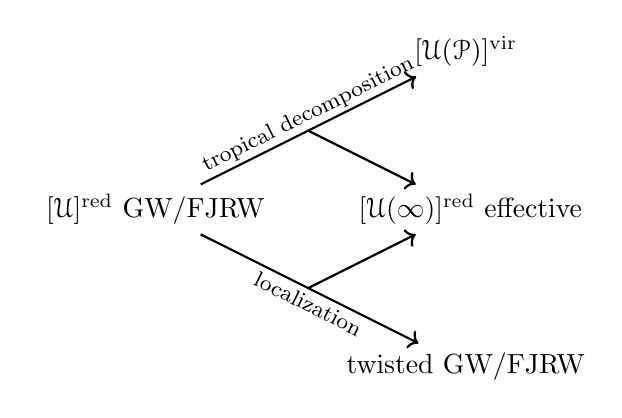
\begin{tikzpicture}[scale=1, transform shape]
    \node (red) at (0,0) {\Centerstack{ {$[\mc{U}]^{\red}$} GW/FJRW }};
    \node (vir) at (4,2) {$[\mc{U}(\mc{P})]^{\vir}$};
    \node (eff) at (4,0) {\Centerstack{ {$[\mc{U}(\infty)]^{\red}$} effective }};
    \node (tw) at (4,-2) {\Centerstack{twisted GW/FJRW}};
    \draw[->,thick] (red) -- (vir); 
    \draw[->,thick] (red) -- (tw); 
    \draw[->,thick] (2,1) -- (eff); 
    \draw[->,thick] (2,-1) -- (eff); 
    \node[rotate=26.5] at (2,1.2) {\footnotesize tropical decomposition};
    \node[rotate=-26.5] at (2,-1.2) {\footnotesize localization};
\end{tikzpicture}
\end{center}
\caption{Relation between structural formulae and virtual cycles in log GLSM}%
\label{fig:structural}
\end{figure}

There are two ways to think about this $\C_{\omega}^{\times}$-action. If we have an $R$-map
\begin{equation*}
\begin{tikzcd}
     & \mf{P} \ar{d} \\
    C \ar[swap]{r}{\omega_C^{\log}} \ar{ur} & B \C_{\omega}^{\times},
\end{tikzcd}
\end{equation*}
this was a morphism of \textbf{stacks}, so there is a $2$-morphism making the diagram commute. Abstractly, the action simply scales the $2$-morphism, which is an isomorphism of line bundles.

More concretely, consider the quintic example. Then an $R$-map is equivalent to the data of a stable map $f \colon C \to \P^4$ and a section of the projective bundle
\[ \P_C (f^* \mc{O}_{\P^4}(-5) \otimes \omega_C^{\log} \oplus \mc{O}_C). \]
Using this description, the $\C_{\omega}^{\times}$-action simply scales the $p$-field, where we scale the first summand and not the second.

We now have a $\C_{\omega}^{\times}$ action on all moduli spaces that we considered previously, for example $\mc{R}(\mf{P}, \beta)$ or $\mc{U}(\mf{P}, \beta)$.

\begin{prop}
    The perfect obstruction theories $\E_{\mc{R}}$ and $\E_{\mc{U}}^{\red}$ are $\C_{\omega}^{\times}$-equivariant.
\end{prop}

\begin{rmk}
    A key input to this result is that the superpotential is $\C_{\omega}^{\times}$-equivariant. If it was in fact invariant, then there would be no need to develop the theory of log GLSM.
\end{rmk}

We may now apply the virtual localization theorem, proved in increasing strength by Graber-Pandharipande, Chang-Kiem-Li, and Aranha-Khan-Latyntsev-Park-Ravi to decompose the reduced virtual cycle as
\[ [\mc{U}]^{\red} = \sum_F \iota_* \frac{[F]^{\red}}{e(N_{F/\mc[U]}^{\vir})}. \]


\subsection{Fixed loci}%
\label{sub:Fixed loci}

There are several kinds of fixed loci:
\begin{itemize}
    \item There is a fixed locus $\mc{R}_{g,\mc{C}}(0_{\mf{P}}, \beta)$ of all maps going into the zero-section.
    \item There is another fixed locus $\mc{R}_{g,\mc{C}}(\infty_{\mf{P}}, \beta)$ of maps going into infinity.
    \item More general fixed loci may be described by decorated bipartite graphs, with vertices at either $0$ or $\infty$ being decorated by a genus and curve class and edges being decorated by the contact order (which implies the degree of the edge).
\end{itemize}
From a bipartite graph, the $R$-maps which appear in the corresponding fixed locus arise from taking scaling limits of $R$-maps of the corresponding tropical type. From the fixed curves, we can obtain other curves of the same tropical type by smoothing nodes which appear at $0$.

The moduli spaces corresponding to stable vertices are given as follows. When $v \in V_{\infty}$, the vertex moduli space is
\[ \mc{R}_v = \mc{R}_{g(v), \mc{C}(v)}(\infty, \beta(v)), \]
where all contact orders are negative. When $v \in V_0$, then we have
\begin{align*}
    \mc{R}_v &= \mc{R}_{g(v), \mc{C}(v)}(0, \beta(V)) \\
    &\cong \mc{M}_v = \Mbar_{g(v), n(v)} (X, \beta(v)),
\end{align*}
where $X$ was the ambient space.

\subsection{Virtual localization formula}%
\label{sub:Virtual localization formula}


\begin{exm}
    In the case of the quintic, note that $\infty \cong 0$. Then we have a stabilization morphism $\on{st} \colon\mc{U} \to \Mbar_{g,n}(X,\beta)$. Then we will describe the virtual localization formula on a moduli space which is related to the fixed locus. It is given by the Cartesian diagram
    \begin{equation*}
    \begin{tikzcd}
        \mc{M}_{\Gamma} \ar{r} \ar{d} & \prod_v \Mbar_v \ar{d}{\ev} \\
        (\P^4)^{|E|} \ar{r}{\Delta} & (\P^4 \times \P^4)^{|E|}.
    \end{tikzcd}
    \end{equation*}
    We then obtain the virtual localization formula
    \begin{align*}
        \on{st}_* [\mc{U}]^{\red} ={}& \sum_{\Gamma} \frac{1}{|\Aut \Gamma|} \iota_{\Gamma,*} \Delta^! \cdot \\
        &\cdot \prod_{v \in V_0} \frac{[\mc{M}_v]^{\vir}}{e^{\C^{\times}}(R\pi_* \omega_C^{\log} \otimes f^* \mc{O}(-5) \otimes \C_{\omega})} \prod_{h \in H_v} \frac{1}{\frac{ t-\ev_h^*(5H) }{c_h} - \psi_h} \\
        &\cdot \prod_{v \in V_{\infty}} \on{st}_* \frac{t [\mc{U}(\infty)]^{\red}}{-t-\psi_{\min}} 
        \cdot \prod_{e} \cdots,
    \end{align*}
    where $t$ is the equivariant parameter and $c_h$ is the contact order. The $0$ part gives the twisted GW theory of $\P^4$ with special insertions and the $\infty$ part gives a more general version of effective invariants.
\end{exm}

\begin{exm}
    In the case of the double cubic, note that $\infty_{\C} \cong \P^5 \times \P^1 \to \P^5 = 0_{\C}$. Then we have a stabilization morphism $\on{st} \colon\mc{U} \to \Mbar_{g,n}(\P^5,\beta)$. For $v \in V_{\infty}$, we have
    \[ \Mbar_v = \Mbar_{g(v), n(v)}(\P^5, \beta(v)) \times_{(\P^5)^{n(v)}} (\P^5 \times \P^1)^{n(v)}. \]
    Then we will describe the virtual localization formula on a moduli space which is related to the fixed locus. It is given by the Cartesian diagram
    \begin{equation*}
    \begin{tikzcd}
        \mc{M}_{\Gamma} \ar{r} \ar{d} & \prod_v \Mbar_v \ar{d}{\ev} \\
        (\P^5 \times \P^1)^{|E|} \ar{r}{\Delta} & (\P^5 \times ( \P^5 \times \P^1 ))^{|E|}.
    \end{tikzcd}
    \end{equation*}
    Here, $\Delta$ is composition the diagonal and deleting the $\P^1$ in the first factor. We then obtain the virtual localization formula
    \begin{align*}
        \on{st}_* [\mc{U}]^{\red} ={}& \sum_{\Gamma} \frac{1}{|\Aut \Gamma|} \iota_{\Gamma,*} \Delta^! \cdot \\
        &\cdot \prod_{v \in V_0} \frac{[\mc{M}_v]^{\vir}}{e^{\C^{\times}}(R\pi_* \omega_C^{\log} \otimes f^* \mc{O}(-3)^{\oplus 2} \otimes \C_{\omega})} \prod_{h \in H_v} \frac{1}{\frac{ t-\ev_h^*(3H+H_{\infty}) }{c_h} - \psi_h} \\
        &\cdot \prod_{v \in V_{\infty}} \on{st}_* \frac{t [\mc{U}(\infty)]^{\red}}{-t-\psi_{\min}} 
        \cdot \prod_{e} \cdots,
    \end{align*}
    where $t$ is the equivariant parameter, $c_h$ is the contact order, and $H_{\infty}$ is the hyperplane class on the $\P^1$ factor. The $0$ part gives the twisted GW theory of $\P^5$ with special insertions and the $\infty$ part gives a more general version of effective invariants.
\end{exm}

\begin{exm}
    In the case of the FJRW theory of the quintic, note that $\infty_C = \sqrt[5]{(\P^4, \mc{O}(1))} \to 0_{\C} = B\mu_5$. Then we have a stabilization morphism $\on{st} \colon\mc{U} \to \Mbar^{\frac{1}{5}}_{g,\mc{C}}$. We now set
    \[ \Mbar_v = \Mbar^{\frac{1}{5}}_{g(v), \mc{C}(v)} \times_{( \bar{I}0_{\C} )^{n(v)}} (\bar{I}\infty_{v})^{n(v)} \]
    Then we will describe the virtual localization formula on a moduli space which is related to the fixed locus. It is given by the Cartesian diagram
    \begin{equation*}
    \begin{tikzcd}
        \mc{M}_{\Gamma} \ar{r} \ar{d} & \prod_v \Mbar_v \ar{d}{\ev} \\
        (\bar{I}\infty_{\C})^{|E|} \ar{r}{\Delta} & (\bar{I}0_{\C} \times \bar{I}\infty_{\C})^{|E|}.
    \end{tikzcd}
    \end{equation*}
    We then obtain the virtual localization formula
    \begin{align*}
        \on{st}_* [\mc{U}]^{\red} ={}& \sum_{\Gamma} \frac{1}{|\Aut \Gamma|} \iota_{\Gamma,*} \Delta^! \cdot \\
        &\cdot \prod_{v \in V_0} \frac{[\mc{M}_v]^{\vir}}{e^{\C^{\times}}(R\pi_* \mc{L} \otimes \C_{\omega})} \prod_{h \in H_v} \frac{1}{\frac{ t-\ev_h^*(H_{\infty}) }{c_h} - \psi_h} \\
        &\cdot \prod_{v \in V_{\infty}} \on{st}_* \frac{5t [\mc{U}(\infty)]^{\red}}{-t-\psi_{\min}} 
        \cdot \prod_{e} \cdots,
    \end{align*}
    where $t$ is the equivariant parameter and $c_h$ is the contact order. The $0$ part gives the twisted GW theory of $\P^4$ with special insertions and the $\infty$ part gives a more general version of effective invariants.
\end{exm}


\section{Applications to Gromov-Witten theory (Shuai Guo and Felix Janda)}%
\label{sec:Calculationslogglsm}

\subsection{Genus two calculations}%
\label{sub:Genus two calculations}

The goal is to prove the formula
\begin{align}
    F_2^{\QM}(Q) ={}& \ab<\ >_2^{t,\QM} - \ab< \frac{-\frac{5}{3}H^3 + \frac{5}{24}H^4t^{-1}}{(t-5H)(t-5H-\psi)}>_1^{t,\QM} \\
    &+ \frac{1}{2} \ab<\frac{-\frac{5}{3}H^3 + \frac{5}{24}H^4 t^{-1}}{(t-5H)(t-5H-\psi)}, \frac{-\frac{5}{3}H^3 + \frac{5}{24}H^4 t^{-1}}{(t-5H)(t-5H-\psi)}>_0^{t,\QM} \label{eqn:c} \\
    &+ \frac{1}{2} \ab<\Delta_* \ab(\frac{\frac{5}{3} H^3 t^{-1}+ \frac{65}{8}H^4 t^{-2}}{(t-5H)^2(5-5H-\psi_1)(5-5H-\psi_2)})>_0^{t,\QM} \label{eqn:d} \\
    &+ F_2(Q=0)
\end{align}
for the quintic threefold.

We will first use the localization formula to compute
\[ \deg [\mc{U}_2(\mf{P}_{X_5}, \beta)]^{\red}. \]
There are many localization graphs, which may be obtained as modifications of the ones in~\Cref{fig:tropgraphs}. The most important ones are displayed in~\Cref{fig:graphs}.
\begin{figure}[htpb]
\begin{center}
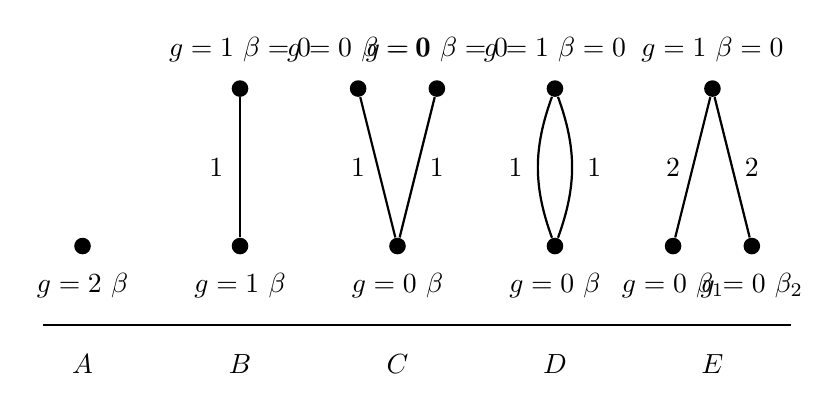
\begin{tikzpicture}[scale=1, transform shape]
    \node[fill=black,circle,minimum size=6pt,inner sep=0pt] (A) at (0,0) {};
    \node[fill=black,circle,minimum size=6pt,inner sep=0pt] (B1) at (2,0) {};
    \node[fill=black,circle,minimum size=6pt,inner sep=0pt] (B2) at (2,2) {};
    \node[fill=black,circle,minimum size=6pt,inner sep=0pt] (C1) at (4,0) {};
    \node[fill=black,circle,minimum size=6pt,inner sep=0pt] (C2) at (3.5,2) {};
    \node[fill=black,circle,minimum size=6pt,inner sep=0pt] (C3) at (4.5,2) {};
    \node[fill=black,circle,minimum size=6pt,inner sep=0pt] (D1) at (6,0) {};
    \node[fill=black,circle,minimum size=6pt,inner sep=0pt] (D2) at (6,2) {};
    \node[fill=black,circle,minimum size=6pt,inner sep=0pt] (E1) at (8,2) {};
    \node[fill=black,circle,minimum size=6pt,inner sep=0pt] (E2) at (7.5,0) {};
    \node[fill=black,circle,minimum size=6pt,inner sep=0pt] (E3) at (8.5,0) {};
    \draw[-,thick] (B1) -- (B2);
    \draw[-,thick] (C2) -- (C1) -- (C3);
    \draw[-,thick] (D1) edge[bend left=20] (D2);
    \draw[-,thick] (D2) edge[bend left=20] (D1);
    \draw[-,thick] (E2) -- (E1) -- (E3);
    \node at (0,-0.5) {\Centerstack{$g=2$ $\beta$}};
    \node at (2,-0.5) {\Centerstack{$g=1$ $\beta$}};
    \node at (4,-0.5) {\Centerstack{$g=0$ $\beta$}};
    \node at (6,-0.5) {\Centerstack{$g=0$ $\beta$}};
    \node at (7.5,-0.5) {\Centerstack{$g=0$ $\beta_1$}};
    \node at (8.5,-0.5) {\Centerstack{$g=0$ $\beta_2$}};
    \node at (2,2.5) {\Centerstack{$g=1$ $\beta=0$}};
    \node at (3.5,2.5) {\Centerstack{$g=0$ $\beta=0$}};
    \node at (4.5,2.5) {\Centerstack{$g=0$ $\beta=0$}};
    \node at (6,2.5) {\Centerstack{$g=1$ $\beta=0$}};
    \node at (8,2.5) {\Centerstack{$g=1$ $\beta=0$}};
    \draw[-,thick] (-0.5,-1) -- (9,-1);
    \node at (0,-1.5) {$A$};
    \node at (2,-1.5) {$B$};
    \node at (4,-1.5) {$C$};
    \node at (6,-1.5) {$D$};
    \node at (8,-1.5) {$E$};
    \node at (1.7,1) {$1$};
    \node at (3.5,1) {$1$};
    \node at (4.5,1) {$1$};
    \node at (5.5,1) {$1$};
    \node at (6.5,1) {$1$};
    \node at (7.5,1) {$2$};
    \node at (8.5,1) {$2$};
\end{tikzpicture}
\end{center}
\caption{Localization graphs with nonzero contribution for $g=2$.}%
\label{fig:graphs}
\end{figure}

The contributions will now be given. For graph $A$, the contribution is
\begin{align*}
    \sum \deg \frac{[\Mbar_2(\P^4, \beta)]^{\vir}}{e(R\pi_* \omega_C^{\log} \otimes f^* \mc[O](-5) \otimes \C_{\omega})} = \ab<\ >_2^t,
\end{align*}
which is the $\mc{O}(5)$-twisted Gromov-Witten potential of $\P^4$. Graph $B$ contributes
\[ \ab<\frac{\ev_* \ab(\frac{[\mc{U}_{1,(-1)}(\infty,0)]^{\vir}}{-t-\psi_{\min}})}{(t-5H)(t-5H-\psi)}>_1^{t} =  \ab< \frac{-\frac{5}{3}H^3 + \frac{5}{24}H^4t^{-1}}{(t-5H)(t-5H-\psi)}>_1^{t}. \]
Graph $C$ contributes~\Cref{eqn:c}, and graph $D$ contributes~\Cref{eqn:d}. Graph $E$ will contribute
\[ c^{\mr{eff}} \cdot \ab<\frac{\cdots}{\frac{t-5H}{2}-\psi}>_0^{t} = F_2(Q=0) \cdot P_1^2(Q), \]
where $c^{\mr{eff}}$ is the effective invariant.


To obtain a formula with five terms from all of our localization graphs, we will apply the shift $\mu = (1-I_0)\psi + I_1 H$ which comes from quasimap wall-crossing. Under the shift, the contribution of graph $E$ becomes the constant $F_2(Q=0)$, while the contributions from all other graphs vanish.
    




\part{See BCOV from the A-side: MSP fields}
\label{pt:msp}


\end{document}

%%% Local Variables:
%%% mode: latex
%%% TeX-master: t
%%% End:
